\documentclass{article}

\usepackage{import} %to nie wiem po co
\usepackage{transparent} %nie pamietam, chyba do odwracania kolorow
\usepackage{xcolor} %nie pamietam, chyba do odwracania kolorow
\usepackage{tcolorbox} %wazne ramki kolorowe
\usepackage{amsmath} %wazne matematyka
\usepackage{upgreek} %nie pamietam, chyba duze litery greckie
\usepackage{alphalph} %zeby numerowanie moglo byc dluzesze niz 50
\usepackage{enumitem} %nie pamietam, chyba to wymieniania
\usepackage{amssymb} %wazne matematyka
\usepackage[margin=0.90in]{geometry} %wazne marginesy
\usepackage{graphicx} %zeby szlo obrazek wkleic

%TO JEST KOMENDA ABY PRZY WYLICZANIU ZACZYNAC OD NOWEJ LINI
\makeatletter
\def\myitem{%
   \@ifnextchar[ \@myitem{\@noitemargtrue\@myitem[\@itemlabel]}}
\def\@myitem[#1]{\item[#1]\mbox{}\\}
\makeatother

%Commands definitions
\newcommand{\setbackgroundcolour}{\pagecolor[rgb]{0.19,0.19,0.19}}  
\newcommand{\settextcolour}{\color[rgb]{0.87,0.87,0.87}}    
\newcommand{\invertbackgroundtext}{\setbackgroundcolour\settextcolour}

%Command execution. 
%If this line is commented, then the appearance remains as usual.
\invertbackgroundtext

%na gorze beda cale komendy usepackage etc

\author{Lukasz Kopyto}
\title{Moje notatki na bazie skryptu topology without tears}

\begin{document}  %begin calego dokumentu
\maketitle     %dowiedz sie o co kaman z tym tytulem, czemu tu jest make

\section{Przestrzenie topologiczne}
\subsection{Topologia: definicje, lematy, zadania i rozwiazania}
\begin{tcolorbox}[colback=white!90!red,colframe=black!35!red,title=1.1.1 Definicja: Topologia]

    Niech $X$ bedzie niepustym zbiorem. Mowimy, ze zbior $T$ zawierajacy podzbiory $X$ jest topologia na $X$ jesli:
    \begin{itemize}
        \item $X$ oraz zbior pusty $\emptyset$, naleza do $T$,
        \item suma skonczona badz nie zbiorow z $T$ nalezy do $T$,
            inaczej $T$ jest zamkniety na sume, i ta suma moze byc nieskonczona
        \item przekroj dowolnych dwoch zbiorow z $T$ nalezy do $T$, inaczej $T$ jest zamkniety na przekroj, ale przekroj skonczony
    \end{itemize}

    Para $(X,T)$ nazywamy \textbf{przestrzenia topologiczna.}
\end{tcolorbox}

\begin{tcolorbox}[colback=white!90!red,colframe=black!35!red,title=1.1.6 Definicja: Topologia dyskretna(discrete topology)]

    Niech $X$ bedzie niepustym zbiorem oraz $T$ kolekcja wszystkich podzbiorow $X$. Wtedy mowimy, ze $T$ jest \textbf{topologia dyskretna} na zbiorze $X$. Przestrzen topologiczna $(X,T)$ jest nazywana \textbf{przestrzenia dyskretna}
\end{tcolorbox}

\begin{tcolorbox}[colback=white!90!red,colframe=black!35!red,title=1.1.7 Definicja: Topologia niedyskretne(indiscrete topology)]

    Niech $X$ bedzie niepustym zbiorem oraz $T= \left\{X, \emptyset\right\}$. Wtedy mowimy, ze $T$ jest \textbf{topologia niedyskretna} oraz $(X,T)$ jest \textbf{przestrzenia niedyskretna} 

\end{tcolorbox}

\begin{tcolorbox}[colback=white!90!green,colframe=black!35!green,title=1.1.9 Lemat: Topologia dyskretna i singletony]

    Jezeli $(X,T)$ jest przestrzenia topologiczna, taka ze, dla kazdego $x \in X$, singleton $x$, $\left\{x\right\}$ jest w $X$, to $X$ jest topologia dyskretna.

\end{tcolorbox}
\textbf{Dowod:}

Wystarcz sprawdzic prawdziwosc trzech warunkow, z definicji $1.1.1$.
\begin{enumerate}
    \item Z definicji $T$ jest topologia, wiec zawiera $X$ oraz $\emptyset$.
    \item Niech $S$ bedzie suma skonczona lub nie dowolnej liczby zbiorow z $T$. Poniewaz mozemy zapisac $S$ jako $S = \bigcup\limits_{x \in S}\left\{x\right\}$, a kazdy singleton $\left\{x\right\} \in X$, wnioskujemy stad, ze $S \in T$ 
    \item Analogicznie dowodzimy, ze przekroj dowolnych dwoch zbiorow z $T$ nalezy do $T$
\end{enumerate}

\hrulefill

\textbf{Cwiczenia 1.1}

\begin{enumerate}
    \item Niech $X = \left\{a,b,c,d,e,f\right\}.$ Ustal czy podane kolekcje podzbiorow $X$ sa topologia na $X$

        \begin{enumerate}[label=(\alph*)]
            \item $T_{1} = \left\{X, \emptyset, \left\{a\right\}, \left\{a,f\right\}, \left\{b,f\right\}, \left\{a,b,f\right\}\right\}$
            \item  $T_{2} = \left\{X, \emptyset, \left\{a,b,f\right\}, \left\{a,b,d\right\}, \left\{a,b,d,f\right\}\right\}$
            \item $T_{3} = \left\{X, \emptyset, \left\{f\right\}, \left\{e,f\right\}, \left\{a,f\right\} \right\}$

        \end{enumerate}
        \textbf{Odpowiedz:}
        \begin{enumerate}[label=(\alph*)]
            \item Jest topologia.
            \item Nie jest, bo $\left\{a,b,f\right\} \cap \left\{a,b,d\right\}= \left\{a,b\right\} \notin T_{2}$ 
            \item Nie jest, bo $\left\{e,f\right\} \cup \left\{a,f\right\}=\left\{a,e,f\right\} \notin T_{3}$ 

        \end{enumerate} 
    \item Niech $X = \left\{a,b,c,d,e,f\right\}.$ Wskaz i uzasadnij ktore kolekcje podzbiorow $X$ sa topologia na $X$

        \begin{enumerate}[label=(\alph*)]
            \item $T_{1} = \left\{X, \emptyset, \left\{c\right\}, \left\{b,d,e\right\}, \left\{b,c,d,e\right\}, \left\{b\right\}\right\}$
            \item  $T_{2} = \left\{X, \emptyset,\left\{a\right\}, \left\{b,d,e\right\}, \left\{a,b,d\right\}, \left\{a,b,d,e\right\}\right\}$
            \item $T_{3} = \left\{X, \emptyset,\left\{b\right\}, \left\{a,b,c\right\}, \left\{d,e,f\right\}, \left\{b,d,e,f\right\} \right\}$

        \end{enumerate}

        \textbf{Odpowiedz:}

        \begin{enumerate}[label=(\alph*)]
            \item Nie, bo $\left\{c\right\} \cup \left\{b\right\} = \left\{b,c\right\} \notin T_{1}$
            \item Nie, bo $\left\{b,d,e\right\} \cap \left\{a,b,d\right\} = \left\{b,d\right\} \notin T_{2}$
            \item Jest topologia.
        \end{enumerate}

    \item Niech $X = \left\{a,b,c,d,e,f\right\}$ oraz $T$ bedzie topologia dyskretna na $X$, ktore z ponizszych podpunktow sa prawdziwe?

        \begin{enumerate}[label=(\alph*)]
            \item $X \in T$- Prawda
            \item $\left\{X\right\} \in T$- Falsz
            \item $\left\{ \emptyset\right\} \in T$- Falsz
            \item $\emptyset \in T$- Prawda
            \item $\emptyset \in X$- Falsz 
            \item $\left\{ \emptyset\right\} \in X$- Falsz
            \item $\left\{a \right\} \in T$- Prawda
            \item $a  \in T$- Falsz
            \item $\emptyset \subseteq X$- Prawda
            \item $\left\{a \right\} \in X$- Falsz
            \item $\left\{\emptyset \right\} \subseteq X$- Falsz
            \item $a \in X$- Prawda
            \item $X \subseteq T$- Falsz
            \item $\left\{a \right\} \subseteq T$- Falsz
            \item $\left\{X\right\} \subseteq T$- Prawda
            \item $a \subseteq T$- Falsz
        \end{enumerate}

    \item Niech $(X, T)$ bedzie dowolna przestrzenia topologiczna. Udowodnij, ze \textbf{przekroj skonczonej liczby(dowolnej) elementow z $T$ jest elementem $T$}

        \textbf{Odpowiedz:}

        Udowodnimy to przez indukcje wzgledem liczby elementow przekroju.

        \textbf{Teza:} Dla przestrzeni topologicznej $(X,T)$ przekroj skonczonej liczby elementow z $T$ jest elementem $T$.

        \textbf{Podstawa indukcji:} dla n = 2, mamy $\bigcap\limits_{i = 1}^{2}A_{i} \text{, gdzie } A_{i} \in T \text{, } A_{i}$ sa dowolnymi zbiorami nalezacymi do $T$. Poniewaz $T$ jest topologia na $X$ wiec z definicji, przekroj dowolnych dwoch zbiorow nalezacych do $T$, nalezy do $T$, zatem $\bigcap\limits_{i = 1}^{2}A_{i} \in T$.

        \textbf{Krok indukcyjny:}
        Ustalmy teraz dowolne $n \in  \mathbb{N}$ i zalozmy, ze $\bigcap\limits_{i = 1}^{n}A_{i} \in T$. Pokaze ze dla $n+1$ teza zachodzi.
        Oznaczmy sobie $B = \bigcap\limits_{i = 1}^{n}A_{i}$.
        Dla $n+1$ mamy:

        $\bigcap\limits_{i = 1}^{n+1}A_{i} = \bigcap\limits_{i = 1}^{n}A_{i} \cap A_{n+1} = \text{ zal. ind. } = B \cap A_{n+1}$
        Poniewaz $B \in T \text{ oraz } A_{n+1} \in T$ wiec z definicji topologi, $B \cap A_{n+1} \in T$  

        Zatem na mocy zasady indukcji matematycznej, dla przestrzeni topologicznej $(X,T)$ przekroj skonczonej liczby elementow z $T$ jest elementem $T$.

    \item Niech $\mathbb{R}$ bedzie zbiorem liczb rzeczywistych. Udowodnij ze kazdy z nastepujacych kolekcji podzbiorow $\mathbb{R}$ jest topologia.

        \begin{enumerate}[label=(\alph*)]
            \item $T_{1}$ zawiera $\mathbb{R}, \emptyset$ oraz kazdy przedzial $(-n, n)$, dla dowolnego $n \in {\mathbb{N}}^{+}$, gdzie $(-n, n)$ oznacza zbior $\left\{x \in \mathbb{R}: -n < x <n\right\}$

            \item $T_{2}$ zawiera $\mathbb{R}, \emptyset$ oraz kazdy przedzial $[-n, n]$, dla dowolnego $n \in {\mathbb{N}}^{+}$, gdzie $[-n, n]$ oznacza zbior $\left\{x \in \mathbb{R}: -n \leq x \leq n\right\}$

            \item $T_{3}$ zawiera $\mathbb{R}, \emptyset$ oraz kazdy przedzial $[n, \infty)$, dla dowolnego $n \in {\mathbb{N}^{+}}$, gdzie $[n, \infty)$ oznacza zbior $\left\{x \in \mathbb{R}: n \leq x\right\}$

        \end{enumerate}

        \textbf{Odpowiedz:}

        Trzeba kazdy podpunkt sprawdzic z definicji topologii, czyli w kazdym podpunkcie sprawdzic czy (a') $X$ oraz $\emptyset$ naleza do $T$, (b') zamknietosc na sume teoriomnogosciowa skonczona lub nie i (c') zamknietosc na przekroj(skonczony)

        \textbf{dla $T_{1}$ mamy:}
        \begin{enumerate}[label=(\alph*')]
            \item Z opisu $T_{1}$ mamy, ze $ \mathbb{R} \in T_{1}$ oraz $\emptyset \in T_{1}$
            \item Niech $U = \bigcup\limits_{\alpha \in A} U_{\alpha}$ gdzie $A_{\alpha} \in T_{1}$ oraz $A$ jest pewnym zbiorem indeksowym, bedzie dowolna suma(skonczona badz nie) zbiorow. Rozwazmy przypadki:
                \begin{itemize}
                    \item $U_{\alpha} = \mathbb{R}$ dla pewnego $\alpha \in A$. 

                        Wtedy $ \bigcup\limits_{\alpha \in A} U_{\alpha} = \mathbb{R} \in T_{1}$
                    \item $U_{\alpha} \neq \mathbb{R}$ dla kazdego $\alpha \in A$.

                        Wtedy mamy przypadki:

                        \begin{itemize}
                            \item $U_{\alpha} = \emptyset$ dla kazdego $\alpha \in A$. 

                                Wtedy $\bigcup\limits_{\alpha \in A} U_{\alpha} = \emptyset \in T_{1}$  
                            \item $U_{\alpha} \neq \emptyset$ dla pewnego $\alpha \in A$ oraz zbior $$B = \left\{n: U_{\alpha} = (-n, n)  \land n \in \mathbb{N} \land \alpha \in A\right\}$$ jest ograniczony z gory.

                                Wtedy, z tego ze zbior $B$ jest ograniczony z gory i zawiera liczby naturalne, wiemy ze istnieje najmniejsza liczba naturalna $m$, ktora ogranicza ten zbior z gory. Wezmy zatem liczbe $m$. Zauwazmy, ze $m$ jest jednoczesnie maximum zbioru B. Z definicji zbioru $T_{1}$ mamy, ze $(-m, m) \in T_{1}$ oraz z tego, ze $B$ jest ograniczony z gory, wnioskujemy $$\bigcup\limits_{\alpha \in A} U_{\alpha} = (-m,m) \in T_{1}$$

                            \item $U_{\alpha} \neq \emptyset$ dla pewnego $\alpha \in A$ oraz zbior $$B = \left\{n: U_{\alpha} = (-n, n) \land n \in \mathbb{N} \land \alpha \in A\right\}$$ jest nieograniczony z gory.

                                Wtedy, mam sprzecznosc, bo zalozylismy, ze $\mathbb{R} \notin T_{1}$, z drugiej strony zbior $B$ jest nieograniczony, a $$\bigcup\limits_{\alpha \in A}U_{\alpha} = \bigcup\limits_{n=1}^{\infty}(-n, n) = \mathbb{R}$$ 
                                Zatem ten podpunkt odpada.

                        \end{itemize}

                        Sprawdzilismy zatem wszystkie mozliwosci i otrzymalismy, ze zbior $T_{1}$ jest zamkniety na sume(skonczona badz nie)

                \end{itemize}
            \item Wezmy dwa dowolne zbiory $B \in T_{1}$ oraz $C \in T_{1}$. Pokazemy, ze $B \cap C \in T_{1}$

                Rozwazmy przypadk:
                \begin{itemize}

                    \item $B \lor C = \emptyset$

                        Wtedy: $B \cap C = \emptyset \in T_{1}$
                    \item $B \land C \neq \emptyset$ Wtedy mamy przypadki:

                        \begin{itemize}

                            \item $B \land C = \mathbb{R}$ 

                                Wtedy $B \cap C = \mathbb{R} \in T_{1}$

                            \item $B \lor C \neq \mathbb{R}$ 

                                Wtedy ktorys ze zbiorow(byc moze oba) jest postaci $(-m,m)$ dla $m \in \mathbb{N}$. Jesli $B = \mathbb{R}$ i $C = (-m,m), m\in \mathbb{N}$ to $B \cap C = (-m,m) \in T_{1}$.
                                Drugi przypadek to gdy oba sa postaci prostej, czyli $B = (-m,m)$ oraz $C = (-n,n)$ dla $m,n \in \mathbb{N}$. Wtedy niech $k = min(m,n)$, mamy $B \cap C = (-k,k) \in T_{1}$

                        \end{itemize}
                \end{itemize}
                Zatem $T_{1}$ zamkniete na przekroj.    
        \end{enumerate}
        $T_{1}$ jest zatem topologia. c.b.d.u.

        \textbf{dla $T_{2}$ mamy:} 

        Dowod bedzie analogiczny do tego z $T_{1}$. Postaram sie go bardziej ladnie zrobic.

        \begin{enumerate}[label=(\alph*')]%poczatek dowodu dla T2

            \item Z opisu $T_{2}$ wnioskujemy, ze $\mathbb{R} \in T_{2}$ oraz $\emptyset \in T_{2}$.
            \item Niech $U = \bigcup\limits_{\alpha \in A}U_{\alpha}$, gdzie $U_{\alpha} \in T_{2}$ oraz $A$ jest pewnym zbiorem indeksowym. Rozwazmy przypadki:

                \begin{itemize}%poczatek pierwszych przypadkow

                    \item $U_{\alpha} = \mathbb{R}$ dla pewnego $\alpha \in A$. Wtedy:

                        $U = \mathbb{R} \in T_{2}$
                    \item $U_{\alpha} \neq \mathbb{R}$ dla kazdego $\alpha \in A$ Wtedy:

                        Rozwazmy przypadki:
                        \begin{itemize}%poczatek drugich przypadkow

                            \item $U_{\alpha} = \emptyset$ dla kazdego $\alpha \in A$ Wtedy:

                                $U = \emptyset \in T_{2}$
                            \item $U_{\alpha} \neq \emptyset$ dla pewnego $\alpha$ Wtedy:

                                Wprowadzmy sobie funkcje zdaniowa $$P(x) = (\exists \alpha \in A)(U_{\alpha} = [-x,x])$$ oraz zbior $$B = \left\{n : P(n) \land n \in \mathbb{N}\right\}$$ jako zbior indeksow $n$ dla ktorych istnieje $\alpha \in A$ taka ze $U_{\alpha} = [-n,n]$.

                                Nastepnie rozwazmy dwa przypadki:

                                I. Zbior $B$ jest ogranioczony z gory.
                                Wtedy z tego, ze $B$ jest ograniczony oraz $B$ zawiera tylko liczby naturalne, wnioskujemy, ze istnieje w $B$ maximum. Niech $m = max(B)$. Wtedy $U = [-m,m] \in T_{2}$ 
                                \vspace{5mm}

                                II. Zbior $B$ jest nieograniczony z gory.
                                Wtedy $U = \bigcup\limits_{\alpha \in A}U_{\alpha} = \bigcup\limits_{n=1}^{\infty}[-n,n] = \mathbb{R}$, lecz zalozylismy, ze $U \neq \mathbb{R}$. Zatem sprzecznosc, wiec ten przypadek nam odpada.

                        \end{itemize}%koniec drugich przypadkow
                        Zatem $T_{2}$ jest zamkniety na sume.

                \end{itemize}%koniec pierwszych przypadkow
            \item Wezmy dowolne dwa zbiory $B \in T_{2}$ oraz $C \in T_{2}$. Wtedy:

                Rozwazmy przypadki:

                \begin{itemize}%poczatek trzecich przypadkow

                    \item $B = \mathbb{R} \land C = \mathbb{R}$. Wtedy:

                        $B \cap C = \mathbb{R} \in T_{2}$.
                    \item WLOG zalozmy, ze $B \neq \mathbb{R}$. Wtedy:

                        Rozwazmy przypadki:
                        \begin{itemize}%poczatek czwartych przypadkow

                            \item $B = \emptyset$. Wtedy bezwzgledu na $C$:

                                $B \cap C = \emptyset \in T_{2}$
                            \item $B = [-n,n]$ dla pewnego $n \in \mathbb{N}$. Wtedy:

                                I. Jesli $C = \emptyset$ to:

                                $B\cap C = \emptyset \in T_{2}$.
                                \vspace{5mm}

                                II. Jesli $C = [-m,m]$ dla pewnego $m \in \mathbb{N}$, Wtedy:

                                Niech $k = min(m, n)$, mamy $B\cap C = [-k,k] \in T_{2}$
                        \end{itemize}%koniec czwartych przypadkow
                        \vspace{5mm}

                        Zatem $T_{2}$ jest zamkniete na skonczone przekroje.  
                \end{itemize}%koniec trzecich przypadkow

                Podsumowujac, sprawdzilismy z definicji topologii i otrzymalismy ze $T_{2}$ jest topologia. c.b.d.u.

        \end{enumerate}%koniec dowodu dla T2

        \textbf{dla $T_{3}$ mamy:}

        \begin{enumerate}[label=(\alph*')] %poczatek dowodu dla T3

            \item Z opisu $T_{3}$ mamy, ze $\mathbb{R} \in T_{3}$ oraz $\emptyset \in T_{3}$
            \item Niech $U = \bigcup\limits_{\alpha \in A}U_{\alpha}$, gdzie $U_{\alpha} \in T_{2}$ oraz $A$ jest pewnym zbiorem indeksowym.

                Wprowadzmy sobie funkcje zdaniowa $$P(x) = (\exists \alpha \in A)(U_{\alpha} = [x, \infty])$$
                oraz zbior
                $$B = \left\{n: P(n) \land n \in {\mathbb{N}}^{+}\right\}$$
                $B$ to zbior wszystkich indeksow $n$ dla ktorych $U_{\alpha} = [n, \infty]$.
                Poniewaz zbior ten zawiera tylko liczby naturalne, wiec ma minimum. Niech $m = min(B)$. Wtedy $U = [m, \infty] \in T_{3}$. Zatem $T_{3}$ jest zamkniety na sume.
            \item Wezmy sobie dowolne zbiory $B \in T_{3}$ oraz $C \in T_{3}$. Niech $b = min(B)$ oraz $c = min(C)$. Wtedy $B\cap C = [min(b,c), \infty] \in T_{3}$ bo $min(b,c) \in \mathbb{N}$. Zatem $T_{3}$ jest zamkniety na przekroj.

                Podsumowujac, rozwazylismy wszystkie mozliwosci i otrzymalsmy, ze $T_{3}$ jest topologia.

        \end{enumerate} %koniec dowodu dla T3

    \item Niech $\mathbb{N}$ bedzie zbiorem liczb naturalnych dodatnich. Udowodnij ze kazda z nastepujacych kolekcji(w ramkach) podzbiorow $\mathbb{N}$ jest topologia.

        \begin{tcolorbox}[colback=white!90!red,colframe=black!35!red,title=Definicja: \textbf{Initial segment topology}; poki co brak polskiego tlumaczenia]
            $T_{1}$ zawiera $\mathbb{N}$ oraz $\emptyset$ oraz kazdy zbior $\left\{1,2,3,\dots,n\right\}$, dla dowolnego $n$ naturalnego dodatniego.
        \end{tcolorbox}
        \textbf{Dowod:}

        \begin{itemize}%poczatek dowodu dla T1 

            \item Z opisu mamy, ze $\emptyset \in T_{1}$ oraz $\mathbb{N} \in T_{1}$
            \item Niech $U = \bigcup\limits_{\alpha \in A}U_{\alpha}$ dla pewnego zbioru indeksowego $A$ i $U_{\alpha} \in T_{1}$. Wprowadzmy sobie funkcje zdaniowa
                $$P(x) = (\exists \alpha \in A)(U_{\alpha} = \left\{1,2,3,\dots,x\right\}$$
                oraz zbior
                $$B = \left\{n: P(n) \land n \in {\mathbb{N}}^{+}\right\}$$
                Rozwazmy przypadki:
                \begin{itemize}%poczatek przypadkow dla sumy

                    \item Zbior $B$ jest ogranioczony z gory.

                        Poniewaz $B$ zawiera liczby naturalne dodatnie i jest ograniczony z gory wiec
                        zawiera maximum. Niech $m = max(B)$. Zatem dla pewnego $\alpha, U_{\alpha} = \left\{1,2,\dots,m\right\}$. Wtedy $U = \left\{1,2,\dots,m\right\} \in T_{1}$.
                    \item Zbior $B$ jest nieograniczony z gory.

                        Poniewaz zbior $B$ zawiera liczby naturalne dodatnie(od 1 wzwyz) i nie jest ograniczony z gory, wiec $B = \mathbb{N}$. Zatem dla dowolnej $\alpha \in A$ istnieje ${\alpha}^{\prime} \in A$ taka ze, $U_{\alpha} \subset U_{{\alpha}^{\prime}}$. Zatem $U = \mathbb{N}$.
                \end{itemize}%koniec przypadkow dla sumy
                Zatem $T_{1}$ jest zamkniety na sume.
            \item Wezmy dowolne dwa zbiory $B \in T_{1}$ oraz $C \in T_{1}$

                Rozwazmy przypadki:
                \begin{itemize}%poczatek przypadkow dla przekroju

                    \item $B = C = \mathbb{N}$. Wtedy:

                        $B\cap C = \mathbb{N} \in T_{1}$
                    \item WLOG $B \neq \mathbb{N}$. Wtedy:

                        Rozwazmy przypadki:
                        \begin{itemize}%poczatek drugich przypadkow dla przekroju

                            \item $B = \emptyset$ Wtedy:

                                Bezwzgledu na $C$. $B\cap C = \emptyset \in T_{1}$
                            \item $B \neq \emptyset$, czyli $B = \left\{1,2,\dots,n\right\}$ dla pewnego $n \in \mathbb{N}$ to:

                                Jesli $C = \emptyset$, to $B\cap C = \emptyset \in T_{1}$.

                                Jesli $C = \left\{1,2,\dots,m\right\}$ dla pewnego $m \in \mathbb{N}$, to $B\cap C = \left\{1,2,\dots,min(n,m)\right\} \in T_{1}$  

                        \end{itemize}%koniec drugich przypadkow dla przekroju
                \end{itemize}%koniec przypadkow dla przekroju
                Zatem $T_{1}$ jest zamkniety na przekroj.

                Zatem $T_{1}$ to topologia.
        \end{itemize}%koniec dowodu dla T1

        \begin{tcolorbox}[colback=white!90!red,colframe=black!35!red,title=Definicja:\textbf{Final segment topology}; poki co brak polskiego tlumaczenia]
            $T_{2}$ zawiera $\mathbb{N}$ oraz $\emptyset$ oraz kazdy zbior $\left\{n, n+1, n+2,\dots \right\}$, dla dowolnego $n$ naturalnego dodatniego.
        \end{tcolorbox}
        \textbf{Dowod:}

        \begin{itemize}%poczatek dowodu dla T2

            \item Z opisu mamy, ze $\emptyset \in T_{2}$ oraz $\mathbb{N} \in T_{2}$
            \item Niech $U = \bigcup\limits_{\alpha \in A}U_{\alpha}$, gdzie $A$ jest pewnym zbiorem indeksowym oraz $U_{\alpha} \in T_{2}$. Wprowadzmy sobie funkcje zdaniowa
                $$P(x) = (\exists \alpha \in A)(U_{\alpha} = \left\{x, x+1, x+2, \dots\right\}$$
                oraz zbior
                $$B = \left\{n: P(n) \land n \in {\mathbb{N}}^{+}\right\}$$

                Niech $m = min(B)$. Wtedy dla kazdego $\alpha \in A, U_{\alpha} \subset \left\{m, m+1, \dots\right\}$ oraz $U = \left\{m, m+1, \dots\right\} \in T_{2}$.

                Zatem $T_{2}$ jest zamkniety na sume.

            \item Wezmy dowolne $B \in T_{2}$ oraz $C \in T_{2}$.

                Rozwazmy przypadki:

                \begin{itemize}%poczatek przypadkow dla przekroju

                    \item $B = \emptyset \lor C = \emptyset$. Wtedy:

                        $B\cap C = \emptyset \in T_{2}$
                    \item $B = \mathbb{N} \land C = \mathbb{N}$. Wtedy:

                        $B\cap C = \mathbb{N} \in T_{2}$

                    \item Zaden z nich nie jest pusty oraz oba nie sa zbiorem $\mathbb{N}$. Wtedy:

                        Jesli $B = \left\{m, m+1, \dots\right\}$ dla pewnego $m \in \mathbb{N}$ oraz $C =  \left\{n, n+1, \dots\right\}$ dla pewnego $n \in \mathbb{N}$, to $B\cap C = \left\{max(m,n), max(m,n)+1, \dots\right\} \in T_{2}$
                        \vspace{5mm}

                        Jesli WLOG $B = \left\{m, m+1, \dots\right\}$ dla pewnego $m \in \mathbb{N}$ oraz $C = \mathbb{N}$ to $B\cap C = \left\{m, m+1, \dots\right\} \in T_{2}$ 
                \end{itemize}%koniec przypadkow dla przekroju
                Zatem $T_{2}$ jest zamkniete na przekroj

                Zatem $T_{2}$ to topologia. c.b.d.u.
        \end{itemize}%koniec dowodu dla T2

    \item Wypisz wszystkie mozliwe topologie na ponizszych zbiorach:

        \begin{enumerate}[label=(\alph*)]%poczatek wymieniania zbiorow z polecenia
            \item $X = \left\{a,b\right\}$

                \textbf{Odpowiedz:}

                Sa takie 4 topologie:
                \begin{enumerate}[label={$T_{\arabic*} = $}]%poczatek wymieniania odpowiedzi

                    \item $\left\{X, \emptyset\right\}$
                    \item $\left\{X, \emptyset, \left\{a\right\}, \left\{b\right\} \right\}$
                    \item $\left\{X, \emptyset, \left\{b\right\} \right\}$
                    \item $\left\{X, \emptyset, \left\{a\right\} \right\}$
                \end{enumerate}%koniec wymieniania odpowiedzi

            \item $X = \left\{a,b,c\right\}$   

                \textbf{Odpowiedz:}

                Jest takich 29 topologii:TODO PRZEPISAC Z KARTKI JE TUTAJ

                TODO NAPISZ DOWOD ZE JEST ICH 29, NA WIKI SPRAWDZ: TOPOLOGIES ON SET WITH 3 ELEMENTS
                \begin{enumerate}[label = {$T_{\arabic*} = $}]%poczatek wymieniania odpowiedzi

                    \item $\left\{X, \emptyset\right\}$
                    \item $\left\{X, \emptyset, \left\{a\right\}, \left\{b\right\}, \left\{c\right\}, \left\{a,b\right\},\left\{a,c\right\},\left\{b,c\right\},\right\}$
                    \item $\left\{X, \emptyset, \left\{a\right\} \right\}$
                    \item $\left\{X, \emptyset, \left\{b\right\} \right\}$
                    \item $\left\{X, \emptyset, \left\{c\right\} \right\}$
                    \item $\left\{X, \emptyset, \left\{a\right\}, \left\{a,b\right\} \right\}$
                    \item $\left\{X, \emptyset, \left\{a\right\}, \left\{a,c\right\} \right\}$
                    \item $\left\{X, \emptyset, \left\{b\right\}, \left\{b,c\right\} \right\}$
                    \item $\left\{X, \emptyset, \left\{b\right\}, \left\{b,a\right\} \right\}$
                    \item $\left\{X, \emptyset, \left\{c\right\}, \left\{c,a\right\} \right\}$
                    \item $\left\{X, \emptyset, \left\{c\right\}, \left\{c,b\right\} \right\}$
                    \item $\left\{X, \emptyset, \left\{a\right\}, \left\{a,b,c\right\} \right\}$
                    \item $\left\{X, \emptyset, \left\{b\right\}, \left\{a,b,c\right\} \right\}$
                    \item $\left\{X, \emptyset, \left\{c\right\}, \left\{a,b,c\right\} \right\}$
                \end{enumerate}%koniec wymieniania odpowiedzi 

        \end{enumerate}%koniec wymieniania zbiorow z polecenia
    \item Udowodnij ponizszy lemat.
        \begin{tcolorbox}[colback=white!90!green,colframe=black!35!green,title=Lemat: Topologia dyskretna i podzbiory nieskonczone]

            Niech $X$ bedzie zbiorem niesoknczonym oraz $T$ topologia na $X$. Jezeli kazdy nieskonczony podzbior $X$ nalezy do $T$, to $T$ jest topologia dyskretna.

        \end{tcolorbox}
        \textbf{Dowod:}

        Zgodnie z ktoryms tam lematem(latwy dowod), jesli $T$ zawiera $\left\{x\right\}$ gdzie $x \in X$ jest dowolnym elementem $X$, to $T$ jest topologia dyskretna. 

        Zatem wezmy dowolny element $x \in X$. Skoro $X$ jest nieskonczonym zbiorem i kazdy nieskonczony podzbior $X$ jest w $T$, to oznacza, ze mozemy sobie wybrac z $X$, nieskonczony ciag roznowartosciowy, w ktorym nie ma elementu $x$. 

        Jak? Na przyklad tak:
        $$
        \begin{cases}
            a_{1} = \begin{cases} 1 \text{ jesli } x \neq 1 \\ 0 \text{ jesli } x = 1   \end{cases} \\
                a_{n} = min\left\{y: y \in X \land y \neq x \land (\forall i \in \left\{1,2,\dots,n-1\right\})(a_{i} \neq y)\right\}
        \end{cases}$$

        Nastepnie rozwazmy dwa nieskonczone zbiory:
        $$A = \left\{a_{n}: n = 2\times k \land k \in \mathbb{Z}\right\} \cup \left\{x\right\}$$
        $$\text{ oraz }$$ 
        $$B = \left\{a_{n}: n = 2\times k + 1\land k \in \mathbb{Z}\right\} \cup \left\{x\right\} $$
        Wtedy oczywiscie $A \in T$ oraz $B \in T$ oraz $A \cap B = \left\{x\right\} \in T$

        Z dowolnosci $x$, wnioskujemy, ze $T$ zawiera dowolny singleton $\left\{x\right\}$ taki ze, $x \in X$. Zatem $T$ jest topologia dyskretna. c.b.d.u. 

    \item Wskaz i udowodnij, ktore z ponizszych zbior liczb rzeczywistych $\mathbb{R}$ sa topologiami.

        \begin{enumerate}[label={$T_{\arabic*} :$}]
            \item zawiera $\mathbb{R}, \emptyset$ oraz kazdy przedzial $(a,b)$ gdzie $a,b \in \mathbb{R}$ oraz $a < b$;

                \textbf{Nie:}

                Wezmy sobie zbior $A = \left\{ 1,2 \right\}$ oraz $B = \left\{ 4,5 \right\}$. Oczywiscie $A \in T_{1}$ oraz $B \in T_{1}$, ale suma $A \cup B = \left\{ 1,2 \right\} \cup \left\{ 4,5 \right\} \notin T_{1}$
            \item zawiera $\mathbb{R}, \emptyset$ oraz kazdy przedzial $(-r,r)$ gdzie $r \in {\mathbb{R}}^{+}$;

                \textbf{Tak:}

                \begin{itemize}
                    \item Z definicjie $\mathbb{R} \in T_{2}$ oraz $\emptyset \in T_{2}$
                    \item Wezmy dowolna $U = \bigcup\limits_{\alpha \in A}U_{\alpha}$, gdzie $U_{\alpha} \in T_{2}$ oraz $A$ jest pewnym zbiorem indeksowym. Wtedy jesli pewien $U_{\alpha} = \mathbb{R}$ to $U = \mathbb{R} \in T_{2}$. W przeciwnym przypadku, jesli kazdy $U_{\alpha} = \emptyset$ to $U = \emptyset \in T_{2}$. W przeciwnym przypadku, jesli nie kazdy $U_{\alpha} = \emptyset$ wtedy rozwazmy przypadki: jesli zbior indeksow $r$, dla ktorych $U_{\alpha} = (-r,r)$, jest ograniczony, to wiemy, ze istnieje indeks $q \in  \mathbb{R}$, taki ze $(\forall \alpha in A)(U_{\alpha} \subseteq (-q,q))$ oraz $(-q,q) \in T_{2}$. Z drugiej strony jesli zbior indeksow $r$, dla ktorych $U_{\alpha} = (-r,r)$, jest nieograniczony, to $U = \mathbb{R} \in T_{2}$. 
                    \item Wezmy dowolne dwa zbiory $A \in T_{2}$ oraz $B \in T_{2}$. Wtedy jesli ktorys z nich jest $\emptyset$ to $A \cap B = \emptyset$. Jesli zaden z nich nie jest $\emptyset$, to albo oba sa $\mathbb{R}$, wtedy $A \cap B = \mathbb{R} \in T_{2}$ albo ktorys z nich nie jest $ \mathbb{R}$. Wtedy albo jeden z nich jest postaci $(-r,r)$ albo oba sa tej postaci, $(-r,r), (-q,q)$. W kazdym przypadku zauwazamy, ze $A \cap B = (-r,r) \in T_{2}$ lub $A \cap B = (-min(r,q), min(r,q)) \in T_{2}$
                \end{itemize}
            \item zawiera $\mathbb{R}, \emptyset$ oraz kazdy przedzial $(-r,r)$ gdzie $r \in {\mathbb{Q}}^{+}$;

                \textbf{Odpowiedz:}

                Nie. Rozwazmy ciag liczb wymiernych $r_{n}$ dazacy do liczby niewymiernej $r$. Dodatkowo rozwazmy nieskonczona sume zbiorow $\bigcup\limits_{i=1}^{\infty}(-r_{n}, r_{n})$. Wtedy przy $n \rightarrow \infty, (-r_{n}, r_{n}) \rightarrow (-r, r)$. Kazdy zbior z  $\bigcup\limits_{i=1}^{infty}(-r_{n}, r_{n})$ jest w $T_{3}$ ale $(-r, r)$ juz nie jest.
            \item zawiera $\mathbb{R}, \emptyset$ oraz kazdy przedzial $[-r,r]$ gdzie $r \in {\mathbb{Q}}^{+}$;

                \textbf{Odpowiedz:}

                Nie. Rozwazmy ciag liczb wymiernych $r_{n}$ dazacy do liczby wymiernej $r$. Dodatkowo rozwazmy nieskonczona sume zbiorow $\bigcup\limits_{i=1}^{\infty}[-r_{n} + \frac{1}{n}, r_{n} - \frac{1}{n}]$. Wtedy przy $n  \rightarrow \infty, [-r_{n} + \frac{1}{n}, r_{n} - \frac{1}{n}] \rightarrow (-r, r)$. Kazdy zbior z sumy  $\bigcup\limits_{i=1}^{\infty}[-r_{n} + \frac{1}{n}, r_{n} - \frac{1}{n}]$ jest w $T_{4}$, ale $(-r, r)$ juz nie jest.
            \item zawiera $\mathbb{R}, \emptyset$ oraz kazdy przedzial $(-r,r)$ gdzie $r \in {\mathbb{R}}^{+} \setminus \mathbb{Q}$;

                \textbf{Odpowiedz:}

                Nie. Rozwazmy ciag liczb niewymiernych dazacy do liczby wymiernej. Niech $r_{n}$ bedzie ciagiem liczb wymiernych dazacym do $\sqrt{2}$. Nastepnie rozwazmy ciag $g_{n} = 2+\sqrt{2} - r_{n}$. Wtedy $\bigcup\limits_{i=1}^{\infty}(-g_{n}, g_{n})$ dazy do $(-2,2)$ przy $n \rightarrow \infty$. Argumentacja podobna jak w przykladzie 4.
            \item zawiera $\mathbb{R}, \emptyset$ oraz kazdy przedzial $[-r,r]$ gdzie $r \in {\mathbb{R}}^{+} \setminus \mathbb{Q}$;

                \textbf{Odpowiedz:}

                Nie. Rozwazmy ciag liczb niewymiernych dazacy do liczby wymiernej $g_{n}$. Rozwazmy nieskonczona sume $\bigcup\limits_{i=1}^{\infty}[-g_{n} + \frac{1}{n}, g_{n} - \frac{1}{n}]$. Suma ta dazy do $[-g, g]$, gdzie $g$ jest liczba wymierna.
            \item zawiera $\mathbb{R}, \emptyset$ oraz kazdy przedzial $[-r,r)$ gdzie $r \in {\mathbb{R}}^{+}$;

                \textbf{Odpowiedz:}

                Nie. Przyklad z podpunktu 4 tutaj zadziala.
            \item zawiera $\mathbb{R}, \emptyset$ oraz kazdy przedzial $(-r,r]$ gdzie $r \in {\mathbb{R}}^{+}$;

                \textbf{Odpowiedz:}
                Nie. Przyklad z podpunktu 4 takza tutaj zadziala.
            \item zawiera $\mathbb{R}, \emptyset$, kazdy przedzial $[-r,r]$ oraz kazdy przedzial $(-r,r)$ gdzie $r \in {\mathbb{R}}^{+}$;

                \textbf{Odowiedz:}

                Tak. Mozna tu zrobic dowod w stylu tych poprzednich- czyli przeanalizowac wszystkie przypadki, ale poczekam na cos lepszego. Zostanie to tutaj uzupelnione.
            \item zawiera $\mathbb{R}, \emptyset$, kazdy przedzial $[-n,n]$ oraz kazdy przedzial $(-r,r)$ gdzie $n \in {\mathbb{N}}^{+}$ oraz  $r \in {\mathbb{R}}^{+}$;

                \textbf{Odpowiedz:}

                Tak. Mozna tu zrobic dowod w stylu tych poprzednich- czyli przeanalizowac wszystkie przypadki, ale poczekam na cos lepszego. Zostanie to tutaj uzupelnione.
        \end{enumerate}


\end{enumerate}%koniec numeracji zadan

\subsection{Zbiory otwarte: definicje, lematy, zadania i rozwiazania}
\begin{tcolorbox}[colback=white!90!red,colframe=black!35!red,title=1.2.1 Definicja: Zbior otwarty- open set]

    Niech $(X, T)$ bedzie przestrzenia topologiczna. Wtedy elementy $T$ nazywaja sie \textbf{zbiory otwarte.}

\end{tcolorbox}

\begin{tcolorbox}[colback=white!90!green,colframe=black!35!green,title=1.2.2 Lemat: Przestrzen topologiczna i zbiory otwarte]
    Niech $(X, T)$ bedzie przestrzenia topologiczna. Wtedy

    \begin{itemize}%poczatek lematu

        \item $X$ oraz $\emptyset$ sa zbiorami otwartymi.
        \item suma(skonczona lub nie) zbiorow otwartych jest zbiorem otwartym
        \item przekroj skonczony zbiorow otwartych jest zbiorem otwartym
    \end{itemize}%koniec lematu
\end{tcolorbox}
\textbf{Dowod:}
Wynika to wprost z definicji. Podpunkt trzeci wynika z zadania 4.

\begin{tcolorbox}[colback=white!90!red,colframe=black!35!red,title=1.2.3 Definicja: Zbior domkniety- closed set]

    Niech $(X,T)$ bedzie przestrzenia topologiczna. Podzbior $S$ zbioru $X$ jest \textbf{zbiorem domknietym} w $(X, T)$ jesli jego dopelnienie w $X$, $X\setminus S$, jest zbiorem otwartym w $(X, T)$
\end{tcolorbox}
\textbf{Komentarz}

Czyli mowimy, ze $S$, bedace podzbiorem $X$, jest zbiorem domknietym w $(X,T)$ jesli jego dopelnienie w $X$, czyli $X\setminus S$ jest otwarte, czli jesli $X\setminus S \in T$

Zauwazmy, ze jesli $(X,T)$ jest przestrzenia dyskretna, wtedy kazdy podzbior $X$ jest zbiorem domknietym. Jednakze w przestrzeni niedyskretnej, $(X,T)$, jedynymi zbiorami domknietymi sa $X$ oraz $\emptyset$

\begin{tcolorbox}[colback=white!90!green,colframe=black!35!green,title=1.2.5 Lemat: Przestrzen topologiczna i zbiory domkniete]

    Niech $(X,T)$ bedzie przestrzenia topologiczna. Wtedy

    \begin{itemize}%poczatek lematu
        \item $\emptyset$ oraz $X$ sa zbiorami domknietymi
        \item przekroj skonczonej lub nieskonczonej liczby zbiorow domknietych jest zbiorem domknietym
        \item suma skonczonej liczby zbiorow zamknietych jest zbiorem domknietym

    \end{itemize}%koniec letmatu
\end{tcolorbox}
\textbf{Komentarz:}

Mozna tu dostrzec pewna analogie pomiedzy przestrzenia topologiczna i zbiorami otwartymi

\textbf{Dowod:}

TODO

\hrulefill


\textbf{Cwiczenie 1.2:}
\begin{enumerate}%poczatek zadan

    \item Wypisz wszystkie 64 podzbiory zbioru $X = \left\{a,b,c,d,e,f \right\}$. Obok kazdego zbioru wypisz czy jest 
        \begin{itemize}
            \item clopen (czyli otwarty i domkniety)
            \item ani domkniety ani otwarty
            \item otwarty ale nie domkniety
            \item domkniety ale nie otwarty
        \end{itemize}
        dla topologii $T$ zadanej na $X$, takiej, ze: $$T = \left\{ X, \emptyset, \left\{ a \right\}, \left\{ c,d \right\}, \left\{ a,c,d \right\}, \left\{ b,c,d,e,f \right\} \right\}$$

        \textbf{Odpowiedz:}
        \begin{enumerate}[label=\arabic*.] %poczatek wymieniania zbiorow

            \item $\emptyset$: jest clopen, bo jest otwarty czyli nalezy do $T$ oraz domkniety bo jego dopelnienie, czyli $X$ nalezy do $T$.
            \item $\left\{ a \right\}$: jest clopen, bo jest otwarty czyli nalezy do $T$ oraz domkniety bo jesgo dopelnienie $\left\{ b,c,d,e,f \right\}$ nalezy do $T$.
            \item $\left\{ b \right\}$: nie jest otwarty bo nie nalezy do $T$ oraz nie jest domkniety, bo jego domkniecie tez nie nalezy do $T$
            \item $\left\{ c \right\}$: nie jest otwarty ani domkniety
            \item $\left\{ d \right\}$: nie jest otwarty ani domkniety
            \item $\left\{ e \right\}$: nie jest otwarty ani domkniety
            \item $\left\{ f \right\}$: nie jest otwarty ani domkniety

            \item $\left\{ a,b \right\}$: nie jest otwarty ani domkniety
            \item $\left\{ a,c \right\}$: nie jest otwarty ani domkniety
            \item $\left\{ a,d \right\}$: nie jest otwarty ani domkniety
            \item $\left\{ a,e \right\}$: nie jest otwarty ani domkniety
            \item $\left\{ a,f \right\}$: nie jest otwarty ani domkniety

            \item $\left\{ b,c \right\}$: nie jest otwarty ani domkniety
            \item $\left\{ b,d \right\}$: nie jest otwarty ani domkniety
            \item $\left\{ b,e \right\}$: nie jest otwarty ani domkniety
            \item $\left\{ b,f \right\}$: nie jest otwarty ani domkniety

            \item $\left\{ c,d \right\}$: jest otwarty bo nalezy do $T$, ale nie jest domkniety bo jego dopasowanie $\left\{ a,b,e,f \right\}$ nie nalezy do $T$
            \item $\left\{ c,e \right\}$: nie jest otwarty ani domkniety
            \item $\left\{ c,f \right\}$: nie jest otwarty ani domkniety

            \item $\left\{ d,e \right\}$: nie jest otwarty ani domkniety
            \item $\left\{ d,f \right\}$: nie jest otwarty ani domkniety

            \item $\left\{ e,f \right\}$: nie jest otwarty ani domkniety

            \item $\left\{ a,b,c \right\}$: nie jest otwarty ani domkniety
            \item $\left\{ a,b,d \right\}$: nie jest otwarty ani domkniety
            \item $\left\{ a,b,e \right\}$: nie jest otwarty ani domkniety
            \item $\left\{ a,b,f \right\}$: nie jest otwarty ani domkniety

            \item $\left\{ a,c,d \right\}$: jest otwarty bo nalezy do $T$, ale nie jest domkniety bo jego dopelnienie $\left\{ b,e,f \right\}$ nie nalezy do $T$
            \item $\left\{ a,c,e \right\}$: nie jest otwarty ani domkniety
            \item $\left\{ a,c,f \right\}$: nie jest otwarty ani domkniety

            \item $\left\{ a,d,e \right\}$: nie jest otwarty ani domkniety
            \item $\left\{ a,d,f \right\}$: nie jest otwarty ani domkniety

            \item $\left\{ a,e,f \right\}$: nie jest otwarty ani domkniety

            \item $\left\{ b,c,d \right\}$: nie jest otwarty ani domkniety
            \item $\left\{ b,c,e \right\}$: nie jest otwarty ani domkniety
            \item $\left\{ b,c,f \right\}$: nie jest otwarty ani domkniety

            \item $\left\{ b,d,e \right\}$: nie jest otwarty ani domkniety
            \item $\left\{ b,d,f \right\}$: nie jest otwarty ani domkniety

            \item $\left\{ b,e,f \right\}$: nie jest otwary, bo nie nalezy do $T$, ale jest domkniety bo jego dopelnienie, czyli $\left\{ a,c,d \right\}$ nalezy do $T$.

            \item $\left\{ c,d,e \right\}$: nie jest otwarty ani domkniety
            \item $\left\{ c,d,f \right\}$: nie jest otwarty ani domkniety

            \item $\left\{ c,e,f \right\}$: nie jest otwarty ani domkniety

            \item $\left\{ d,e,f \right\}$: nie jest otwarty ani domkniety

            \item $\left\{ a,b,c,d \right\}$: nie jest otwarty ani domkniety
            \item $\left\{ a,b,c,e \right\}$: nie jest otwarty ani domkniety
            \item $\left\{ a,b,c,f \right\}$: nie jest otwarty ani domkniety

            \item $\left\{ a,b,d,e \right\}$: nie jest otwarty ani domkniety
            \item $\left\{ a,b,d,f \right\}$: nie jest otwarty ani domkniety

            \item $\left\{ a,b,e,f \right\}$: nie jest otwarty bo nie nalezy do $T$, ale jest domkniety bo jego dopelnienie czyli ${c,d}$ nalezy do $T$

            \item $\left\{ a,c,e,f \right\}$: nie jest otwarty ani domkniety 

            \item $\left\{ a,c,d.e \right\}$: nie jest otwarty ani domkniety
            \item $\left\{ a,c,d,f \right\}$: nie jest otwarty ani domkniety

            \item $\left\{ a,c,e,f \right\}$: nie jest otwarty ani domkniety
            \item $\left\{ a,d,e,f \right\}$: nie jest otwarty ani domkniety
            \item $\left\{ b,c,d,e \right\}$: nie jest otwarty ani domkniety
            \item $\left\{ b,c,d,f \right\}$: nie jest otwarty ani domkniety
            \item $\left\{ b,c,e,f \right\}$: nie jest otwarty ani domkniety
            \item $\left\{ b,d,e,f \right\}$: nie jest otwarty ani domkniety
            \item $\left\{ c,d,e,f \right\}$: nie jest otwarty ani domkniety
            \item $\left\{ a,b,c,d,e \right\}$: nie jest otwarty ani domkniety
            \item $\left\{ a,b,c,d,f \right\}$: nie jest otwarty ani domkniety
            \item $\left\{ a,b,d,e,f \right\}$: nie jest otwarty ani domkniety
            \item $\left\{ a,c,d,e,f \right\}$: nie jest otwarty ani domkniety
            \item $\left\{ b,c,d,e,f \right\}$: jest clopen, bo nalezy do $T$ oraz jest domkniety bo jego dopelnienie $\left\{ a \right\}$ nalezy do $T$
            \item $\left\{ a,b,c,d,e,f \right\}$: jest clopen, nalezy do $T$ oraz jest domkniety bo jego dopelnienie czyli $\emptyset$ nalezy do $T$

        \end{enumerate} %koniec wymieniania zbiorow
    \item Niech $(X,T)$ bedzie przestrzenia topologiczna z wlasnoscia taka, ze kazdy podzbior jest domkniety(closed). Udowodnij ze jest to przestrzen dyskretna.

        \textbf{Odpowiedz:}

        Zauwazmy ze przestrzen dyskretna to taka przestrzen, ktora zawiera wszystkie swojw podzbiory, rownowaznie zawiera kazdy singleton.
        Z zalozen zadania mamy, ze kazdy podzbior $X$ jest domkniety. Wezmy dowolny podzbior $X$, nazwijmy go $A$. Skoro kazdy podzbior $X$ jest domkniety oraz $X \setminus A \subseteq X$, wnioskujemy, ze $X \setminus A$ jest domkniety, czyli jego dopelnienie, czyli $A$ jest otwarte. Z dowolnosci wyboru $A$, mamy, ze $(X,T)$ jest przestrzenia dyskretna.

    \item Pokaz ze jesli $(X,T)$ jest przestrzenia dyskretna lub przestrzenia nie dyskretna, wtedy kazdy otwarty(open) zbior jest clopen zbiorem. Znajdz topologia $T$ na zbiorze $X = \left\{ a,b,c,d \right\}$, ktora nie jest dyskretna oraz nie jest nie dyskretna ale ma wlasnosc taka, ze kazdy zbior otwarty(open) jest clopen.

        \textbf{Odpowiedz:}

        Zalozmy, ze $(X,T)$ jest przestrzenia topologiczna taka, ze kazdy jej podzbior jest domkniety. Skoro kazdy podzbior jest domkniety, to kazdy podzbior jest otwarty. Czyli kazdy podzbior $X$ nalezy do $T$. Zatem $(X,T)$ jest przestrzenia dyskretna. 

    \item Niech $X$ bedzie zbiorem nieskonczonym. Jesli $T$ jest topologia na $X$ taka ze kazdy nieskonczony podzbior $X$ jest domkniety(closed), udowodnij ze $T$ jest topologia dyskretna.

        \textbf{Odpowiedz}

        Mamy, ze $X$ jest zbiorem nieskonczonym oraz topologia $T$ na $X$ ma taka wlasnosc, ze kazdy nieskonczony podzbior $X$ jest domkniety. Wezmy dowolny element $a \in X$, rozwazmy nieskonczony zbior $X\setminus \left\{ a \right\}$. Jest on oczwyscie nieskonczony i jest podzbiorem $X$. Zatem jest domkniety, czyli jego dopelnienie- $\left\{ a \right\} \in T$. Poniewaz $a$ bylo dowolnym elementem $X$, wnioskujemy, ze $T$ jest topologia dyskretna.

    \item Niech $X$ bedzie nieskonczonym zbiorem oraz $T$ topologia na $X$ z wlasnoscia taka, ze jedynym nieskonczonym podzbiorem $X$, ktory jest otwarty jest $X$. Czy $(X, T)$ musi byc przestrzenia niedyskretna?

        \textbf{Odpowiedz:}

        Nie. Wezmy $X = \mathbb{N}$ oraz topologie $T$ na $X$: $T = \left\{ \mathbb{N}, \emptyset, \left\{ 1,2 \right\} \right\}$. TODO 

    \item Niech $T$ bedzie topologia na zbiorze $X$ taka, ze ma tylko 4 zbiory; dokladnie, $T = \left\{ X, \emptyset, A, B \right\}$ gdzie $A$ i $B$ to niepuste rozne, podzbiory \textbf{wlasciwe}(czyli nie moga byc rowne $X$) $X$.

        Udowodnij ze $A$ i $B$ spelniaja tylko jeden z wymienionych kryteriow:
        \begin{itemize}
            \item $B = X \setminus A$;
            \item $A \subset B$;
            \item $B \subset A$.
        \end{itemize}

        Korzystajac z powyzszego zadania, wypisz wszystkie topologie na $X = \left\{ 1,2,3,4 \right\}$ zawierajace dokladnie 4 zbiory.

    \item
        \begin{itemize}
            \item Uzywajac indukcji, udowodnij ze wraz ze wzrostem $n$, gdzie n to liczba elementow zbioru $X$, liczba topologii na zbiorze $X$ wzrasta.
            \item Uzywajac indukcji udowonij ze jesli skonczony zbior $X$ ma $n \in \mathbb{N}$ punktow, to ma conajmniej $(n-1)!$ roznych topologii.
            \item Jesli zbior $X$ jest dowolnym nieskonczonym zbiorem o mocy(cardinality) $\aleph$, czyli jest przeliczalny. Udowodnij, ze jest conajmniej $2^{\aleph}$ roznych topologii na $X$. Wywnioskuj ze kazdy nieskonczony zbior ma nieprzeliczlanie duzoe roznych topologii na sobie.
        \end{itemize}
\end{enumerate}%koniec zadan
\subsection{Skonczenie-domknieta topologia(ang. The Finite-Closed Topology): definicje lematy, zadania i rozwiazania.}

Do tej pory definiowalismy topologie poprzez okreslanie ktore zbiory sa otwarte. Czasami jest bardziej naturalnie opisac topologie poprzez okreslenie ktore zbiory sa domkniete. 

\begin{tcolorbox}[colback=white!90!red,colframe=black!35!red,title=1.3.1 Definicja: Skonczenie domknieta topologia(finite-closed topology(cofinite topology))]

    Niech $X$ bedzie nie pustym zbiorem. Mowimy ze topologia $T$ na $X$ jest \textbf{skonczenie-domknieta topologia lub koskonczona topologia}(ang. finite-closed topology or cofinite topology) jesli domknietymi podzbiorami $X$ sa $X$ oraz wszystkie skonczone podzbiory $X$; czyli otwartymi zbiorami sa $\emptyset$ oraz wszystkie podzbiory $X$, ktore maja skonczone dopelnienia.

    Inaczej:

    $$T = \left\{ A \subseteq X: A = \emptyset \text{ or }X \setminus A\text{ jest skonczony} \right\}$$
\end{tcolorbox}

\textbf{Dowod, ze T z tej definicji jest rzeczywiscie topologia} TODO

\textbf{Komentarz:}

Zauwazmy, ze definicja 1.3.1 nie mowi nam, ze kazda topologia ktora zawiera w sobie $X$ oraz domkniete skonczone podzbiory $X$ jest skonczenie-domknieta topologia. Chodzi o to, ze domknietymi zbiorami musza byc tylko skonczone podzbiory $X$. W skonczenie-wymiarowej topologi wszystkie skonczone zbiory sa domkniete. Jednakze ponizszy przyklad pokazuje ze nieskonczone podzbiory nie musza byc otwarte.

\textbf{1.3.2 Przyklad} Rozwazmy zbior $\mathbb{N}$. Wtedy zbiory $\left\{ 1 \right\}, \left\{ 5,6,7 \right\}, \left\{ 2,4,6,8 \right\}$ sa skonczone wiec sa domkniete w skonczenie-domknietej topologii. Zatem ich dopelnienia:
$$\left\{ 2,3,4,\dots \right\}, \left\{ 1,2,3,4,8,9,\dots \right\}, \left\{ 1,3,5,7,\dots \right\}$$ sa otwarte w skonczenie-domknietej topologii. Z drugiej strony, zbior parzystych liczb naturalnych nie jest domknietem zbiorem poniewaz nie jest skonczony wiec jego dopelnienie, zbior liczb nieparzystych nie jest zbiorem domknietym w skonczenie-wymiarowej topologii. Wiec wszystkie skonczone zbiory sa domkniete, ale nie wszystkie nieskonczone zbiory sa otwarte. 

\textbf{1.3.3 Przyklad}

Niech $T$ bedzie skonczenie-wymiarowa topologia na zbiorze $X$. Jesli $X$ ma przynajmniej 3 rozne clopen podzzbiory, udowodnij ze $X$ jest skonczonym zbiorem.

\textbf{Komentarz do przykladu:}

W zalozeniach zadania przykladu mamy to, ze $T$ jest \textbf{skonczenie-domknieta topologia} oraz ze sa conajmniej 3 rozne clopen zbiory.
Mamy pokazac, ze $X$ jest zbiorem skonczonym.

Przypomnijmy, ze $T$ jest \textbf{skonczenie-domknieta topologia}, czyli znaczy to ze rodzina wszystkich domknietych zbiorow sklada sie z $X$ oraz wszystkich skonczonych podzbiorow $X$. Przypominjmy rowniez, ze zbior jest clopen wtedy i tylko wtedy jesli jest jednoczesnie otwarty(open) oraz domkniety(closed).
Przypomnijmy rowniez ze w kazdej przestrzeni topologicznej sa przynajmniej 2 zbiory, ktore sa clopen, mianowicie $X$ oraz $\emptyset$. W przykladzie mamy dodatkowo podane, ze w przestrzeni $(X,T)$ sa conajmniej 3 zbiory, ktore sa clopen. Wynika z tego, ze jest jeszcze jeden zbior clopen, ktory jest rozny od $X$ oraz $\emptyset$.

\textbf{Dowod:}

Przestrzen topologiczna $(X,T)$ ma 3 rozne podzbiory, ktore sa clopen, wiemy ze jest pewien podzbior $S \subseteq X$ taki ze, $S \neq X$ oraz $S \neq \emptyset$. Poniewaz $S$ jest otwarty w $(X, T)$, wiec jego dopelnienie $X \setminus S$ jest zbiorem domknietym. Wiec $S$ oraz $X \setminus S$ sa domkniete w skonczenie domknietej topologi $T$. Zatem $S$ oraz $X \setminus S$ sa obaj skonczonymi zbiorami, ponieaz zaden z nich nie jest rowny $X$. Ale $X = S \cup X\setminus S$, wiec $X$ jest suma dwoch skonczonych zbiorow. Zatem $X$ jest zbiorem skonczonym.


\textbf{WDM-powtorka:}
\hrule

\begin{tcolorbox}[colback=white!90!red,colframe=black!35!red,title=1.3.4 Definicja: Funkcja injekcja/surjekcja/bijekcja]
    Niech f bedzie funkcja z zbioru $X$ w zbior $Y$.
    \begin{itemize}
        \item Funkcja f jest 1-1 lub injekcja jesli $$ f(x_{1}) = f(x_{2}) \rightarrow x_{1} = x_{2}, \text{ dla } x_{1},x_{2} \in X$$
        \item Funkcja f jest na lub surjekcja jesli $$ (\forall y \in Y)(\exists x \in X)(f(x) = y)$$
        \item Funkcja f jest bijekcja jesli jest jednoczesnie 1-1 i na.
    \end{itemize}
\end{tcolorbox}

\begin{tcolorbox}[colback=white!90!red,colframe=black!35!red,title=1.3.5 Definicja: Odwrotnosc funkcji.]

    Niech f bedzie funkcja z zbioru $X$ w zbior $Y$. Mowimy, ze funkcja f ma odwrotnosc($\textbf{have an inverse}$) jesl istnieje taka funkjca g z $Y$ w $X$, ze $g(f(x)) = x$, for all $x \in X$ oraz $f(g(y)) = y$, for all $y \in Y$. Funkcje g nazywamy funkcja odwrotna($\textbf{inverse function}$) do f. 
\end{tcolorbox}

\begin{tcolorbox}[colback=white!90!green,colframe=black!35!green,title=1.3.6 Lemat: Wlasnosci funkcji.]
    Niech f bedzie funkcja z zbioru $X$ w zbior $Y$.
    \begin{itemize}
        \item Funkcja f ma odwrotnosc iff f jest bijekcja
        \item Niech $g_{1}$ oraz $g_{2}$ beda funkcjami z $Y$ w $X$. Jesli $g_{1}$ oraz $g_{2}$ sa obie funkcjami odwrotnymi do f, wtedy $g_{1} = g_{2}$; to znaczy $g_{y} = g_{y}$, dla kazdego $y \in Y$.
        \item Niech  g bedzie funkcja z $Y$ w $X$. Wtedy g jest funkcja odwrotna do f iff f jest funkcja odwrotna do g.
    \end{itemize}
\end{tcolorbox}

\textbf{Dowod:} TODO

Bardzo wazna definicja.
\begin{tcolorbox}[colback=white!90!red,colframe=black!35!red,title=1.3.7 Definicja: Przeciwobraz funkcji]

    Niech f bedzie funkcja ze zbioru $X$ w zbior $Y$. Jesli $S$ jest dowolnym podzbiorem $Y$, to zbior $f^{-1}(S)$ jest zdefiniowany jako:
    $$f^{-1}(S) = \left\{ x: x \in X \text{ and } f(x) \in S \right\}$$
    Mowimy, ze podzbior $f^{-1}(S)$ zbioru $X$ jest przeciwobrazem($\textbf{inverse image}$) zbioru S(przy odwzorowaniu f).

\end{tcolorbox}

\textbf{Komentarz:}

Zauwazmy ze funkcja odwrotna do funkcji $f: X \rightarrow Y$ istnieje iff f jest bijekcja. Natmiast przeciwobraz dowolnego podzbioru $Y$ istnieje nawet wtedy, kiedy f nie jest 1-1 ani na.

Konczymy ten rozdzial ciekawym przykladem.

\textbf{1.3.9 Przyklad}

Niech $(Y,T)$ bedzie przestrzenia topologiczna oraz $X$ niepustym zbiorem. Niech f bedzie funkcja z $X$ w $Y$. Polozmy $T_{1} = \left\{ f^{-1}(S) : S \in T \right\}$. Udowodnij, ze $T_{1}$ jest topologia na $X$.

\textbf{Dowod:}

Musimy pokazac zachodzenie trzech podpunktow z definicji topologii.
\begin{itemize}
    \item

        \begin{gather}        
            X \in T_{1} \hspace{5mm} \text{ bo } \hspace{5mm} X = f^{-1}(Y)\hspace{5mm}  \text{ i } \hspace{5mm} Y \in T \\ 
            \emptyset \in T_{1} \hspace{5mm} \text{ bo } \hspace{5mm} \emptyset = f^{-1}(\emptyset) \hspace{5mm} \text{ i } \hspace{5mm} \emptyset \in T
        \end{gather}
        Zatem $T_{1}$ ma wlasnosc nr 1.
    \item  Niech $\left\{ A_{j}: j \in J \right\}$ bedzie kolekcja elementow z $T_{1}$, dla jakiegos zbioru indekoswego $J$. Pokazemy, ze $\bigcup\limits_{j \in J}A_{j} \in T_{1}$. Poniewaz $A_{j} \in T_{1}$, wiec z definicji $T_{1}$ wynika, ze $A_{j} = f^{-1}(B_{j})$, gdzie $B_{j} \in T$. Ponadto $ \bigcup\limits_{j \in J}A_{j} = \bigcup\limits_{j \in J}f^{-1}(B_{j}) = f^{-1}(\bigcup\limits_{j \in J}B_{j})$.(Dowod w cw 1.3 $\#1$)
        Zauwazmy ze $B_{j} \in T$, dla kazdego $j \in J$, wiec $\bigcup\limits_{j \in J}B_{j}$, bo $T$ jest topologia na $Y$. Zatem z definicji $T_{1}$, $f^{-1}(\bigcup\limits_{j \in J}B_{j}) \in T_{1}$; czyli $\bigcup\limits_{j \in J}A_{j} \in T_{1}$. Zatem $T_{1}$ ma wlasnosc numer 2. 
    \item Niech $A_{1}$ oraz $A_{2}$ beda w $T_{1}$. Musimy pokazac, ze $A_{1} \cap A_{2} \in T_{1}$. Poniewaz $A_{1}, A_{2} \in T_{1}$, $A_{1} = f^{-1}(B_{1})$ oraz $A_{2} = f^{-1}(B_{2})$, gdzie $B_{1}, B_{2} \in T$. $A_{1} \cap A_{2} = f^{-1}(B_{1})\cap f^{-1}(B_{2}) = f^{-1}(B_{1} \cap B_{2}$. (Dowod w cw 1.3 $\#$1).
        Poniewaz $B_{1} \cap B_{2} \in T$, mamy $f^{-1}(B_{1} \cap B_{2}) \in T_{1}$. Zatem $A_{1} \cap A_{2} \in T_{1}$ i pokazalismy ze $T_{1}$ spelnia wlasnosc nr 3 z definicji topologii.
\end{itemize}
Zatem $T_{1}$ jest rzeczywiscie topologia.

\textbf{Komentarz, bardzow wazny:}

Odnosi sie do punktu drugiego definicji topologii, w ktorej musimy pokazac ze dowolna suma(skonczone lub nie) zbiorow z T, nalezy do T. Otoz nie kazde zbiory sa przeliczalne. Wiec nie wystarczy zaklozyc, ze zbiory $A_{1}, A_{2}, \dots, A_{n}, \dots$ sa w $T_{1}$ i pokazac ze ich suma tez jest w $T_{1}$. To dowiedzie tylko temu, ze \textbf{przeliczalna} suma zbiorow z $T$, nalezy do $T$. Nie wystarczy to aby pokazac wlasnosc nr 2. Wlasnosc ta wymaga aby \textbf{dowolna} suma zbiorow z $T$ skonczona lub nie, przeliczalna lub nie przeliczalna, nalezala do $T$. 

\hrulefill

\textbf{Cwiczenia 1.3}



\begin{enumerate}[align=left] %poczatek zadan 1.3
        \renewcommand{\labelenumi}{\textbf{Cwiczenie 1.3.\arabic{enumi}}}
    \item \hfill \newline Niech f bedzie funkcje z zbioru $X$ w zbior $Y$. W przykladzie 1.3.9 powiedzielismy, ze:

        $$(1): \hspace{1cm} f^{-1}(\bigcup\limits_{j \in J}B_{j}) = \bigcup\limits_{j \in J}f^{-1(B_{j})} $$

        oraz

        $$(2): \hspace{1cm} f^{-1}(B_{1} \cap B_{2}) = f^{-1}(B_{1})\cap f^{-1}(B_{2})$$
        Dla dowolnych podzbiorw $B_{j} \subseteq Y$ oraz dowolnego zbioru indeksowego J.
        \begin{enumerate}[label=(\alph*)]
            \item Udowodnij (1)
            \item Udowodnij (2)
            \item Podaj przyklad zbiorow $A_{1}, A_{2}, X, Y$ oraz funkcji $f: X \rightarrow Y$ takich ze:
                $$f(A_{1} \cap A_{2}) \neq f(A_{1}) \cap f(A_{2})$$
                gdzie $A_{1} \subseteq X, A_{2} \subseteq Y$
        \end{enumerate}

        \myitem Rozstrzygnij czy topologia $T$ w cwiczeniu 1.1.6 jest skonczenie-domknieta topologia.(Udowodnij odpowiedz)

        \myitem Mowimy ze przestrzen topologiczna $(X,T)$ jest \textcolor{red}{$T_{1}$-przestrzenia} jesli kazdy singleton $ \left\{x \right\}$ jest domkniety w $(X,T)$. Pokaz i udowodnij ze dokladnie dwie z kolejnych dziewieciu przestrzeni topologicznych sa $T_{1}-przestrzeniami$.
        \begin{enumerate}[label=(\alph*)] %poczatek z zadania 1.3.3
            \item przestrzen dyskretna
            \item przestrzen nie dyskretna z conajmniej dwoma punktami
            \item zbior nieskonczony z skonczenie-domknieta topologia
            \item przyklad 1.1.2
            \item przyklad 1.1.5 (i)
            \item przyklad 1.1.5 (ii)
            \item przyklad 1.1.5 (iii)
            \item przyklad 1.1.6 (i)
            \item przyklad 1.1.6 (ii)
        \end{enumerate} %koniec z zadania 1.3.3

        \myitem Niech $T$ bedzie skonczenie-domknieta topologia na zbiorze $X$. Jesli $T$ jest dodatkowo topologia dyskretna, to udowodnij ze zbior $X$ jest skonczony.
        \myitem Mowimy ze przestrzen topologiczna $(X,T)$ jest \textcolor{red}{$T_{0}$-przestrzenia} jesli dla kazdej pary roznych punktow a,b w $X$, albo istnieje zbior otwarty zawierajacy a ale nie b albo istnieje zbior otwarty zawierajacy b ale nie a.

        \begin{enumerate}[label=(\alph*)]
            \item Udowodnij ze kazda $T_{1}$-przestrzen jest tez $T_{0}$- przestrzenia.
            \item Ktore przestrzenie z cwiczenia 1.3.3 sa $T_{0}$-przestrzeniami. Uzasadnij swoje odpowiedzi.
            \item Zdefiniuj?Stworz? topologie $T$ na zbiorze $X = \left\{ 0,1 \right\}$ tak ze $(X,T)$ bedzie $T_{0}$-przestrzenia, ale nie $T_{1}$-przestrzenia. Nazywa sie taka przestrzen \textcolor{red}{przestrzenia Sierpinskiego}.
            \item Udowodnij ze kazda przestrzen topologiczna opisana w cwiczeniu 1.1.6 jest $T_{0}$-przestrzenia
            
        \end{enumerate}
    \myitem \textcolor{red}{przeliczalnie-domknieta topologia} (ang. countable-closed topology).
        Niech $X$ bedzie zbiorem nieskonczonym. Przeliczalnie-domknieta topologia jest zdefiniowana jako topologia ktora jak zbiory domkniete ma $X$ oraz wszystkie przeliczalnie podzbiory $X$. Udowodnij ze jest to topologia na $X$.
         
        \myitem \textcolor{red}{Przekroj dwoch topologii}
        Niech $T_{1}$ oraz $T_{2}$ beda dwoma topologiami na zbiore $X$. Udowodnij nastepujace twierdzenia.

        \begin{enumerate}[label=(\alph*)]
            \item jesli $T_{3} = T_{1} \cup T_{2}$, wtedy $T_{3}$ nie jest zawsze topologia na $X$
            \item jesli $T_{4}$ jest zdefiniowana jako $T_{4} = T_{1} \cap T_{2}$ to wtedy $T_{4}$ jest topologia na $X$. Mowimy ze jest to przekroj topologii $T_{1}$ i $T_{2}$
            \item jesli $(X, T_{1})$ oraz $(X, T_{2})$ sa $T_{1}$-przestrzeniami, wtedy $(T_{4}, X)$ jest $T_{1}$-przestrzenia
            \item jesli $(X, T_{1})$ oraz $(X, T_{2})$ sa $T_{0}$-przestrzeniami, wtedy $(T_{4}, X)$ nie jest koniecznie $T_{0}$-przestrzenia
            \item jesli $T_{1}, T_{2}, \dots, T_{n}$ sa topologiami na $X$ to wtedy $T = \bigcap\limits_{i=1}^{n} T_{i}$ jest topologia na $X$.
            \item jesli dla kazdego $i \in I$, gdzie zbior $I$ jest jakims zbiorem indeksowym, kazde $T_{i}$ jest topologia na zbiorze $X$, to wtedy $T = \bigcap\limits_{i \in I} T_{i}$ jest topologia na $X$.
 
        \end{enumerate}

        \myitem \textcolor{red}{Rozne $T_{0}$-topologie na skonczonym zbiorze}
        Udowodnij uzywajac indukcji, ze wraz ze wzrostem n, liczba $T_{0}$-przestrzeni wzrasta.
        \myitem \textcolor{red}{przestrzen drzwiowa(door space)}
        Mowimy ze przestrzen topologiczna $(X,T)$ jest przestrzenia drzwiowa(door space) jesli kazdy podzbior $X$ jest albo otwrtym zbiorem albo domknietym albo oba(clopen).

        \begin{enumerate}[label=(\alph*)]
            \item czy przestrzen dyskretna jest przestrzenia drzwiowa
            \item czy przestrzen niedyskretna jest przestrzenia drzwiowa
            \item jesli $X$ jest zbiorem nieskonczonym oraz $T$ skonczenie-domknieta topologia, to czy $(X,T)$ jest przestrzenia drzwiowa?
            \item niech $X$ bedzie zbiorem $\left\{ a,b,c,d \right\}$. Wypisz/zidentyfikuj te tpologie $T$ na $X$, ktore sa przestrzeniami drzwiowymi??
            
        \end{enumerate}
        \myitem \textcolor{red}{zbiory nasycone(saturated sets)}
        Mowimy ze podzbior $S$ przestrzeni topologiczne $(X,T)$ jest \textcolor{red}{nasycony} jesli jest przekrojem zbiorow otwartych w $(X,T)$.

        \begin{enumerate}[label=(\alph*)]
            \item sprawdz ze kazdy zbior otwarty jest nasycony
            \item sprawdz ze w $T_{1}$-przestrzeni kazdy zbior jest nasycony
            \item podaj przyklad przestrzeni topologicznej ktora ma conajmniej jeden podzbior ktory nie jest nasycony
            \item czy prawda jest ze jesli przestrzen topologiczna $(X,T)$ ma wlasnosc taka, ze kazdy jej podzbior jest nasycony, to jest ona wtesy $T_{1}$-przestrzenia?
            
        \end{enumerate}
\end{enumerate}%koniec zadan 1.3

\section{Topologia euklidesowa}
\subsection{Topologia euklidesowa na $\mathbb{R}$}

\begin{tcolorbox}[colback=white!90!red,colframe=black!35!red,title=2.1.1 Definicja: Topologia euklidesowa na $\mathbb{R}$]
    Mowimy ze podzbior $S$ zbioru $\mathbb{R}$ jest otwarty w \textbf{topologii euklidesowej na $\mathbb{R}$} jesli spelnia nastepujace wlasnosci:
    $$(*)(\forall x \in S)(\exists a,b \in \mathbb{R}\land a<b)(x \in (a,b) \subseteq S)$$

    Czyli dla kazdego $x \in S$, istnieja $a,b \in \mathbb{R}$, $a<b$, takie ze $x \in (a,b) \subseteq S$

    Wlasnymi slowami, dla kazdego elementu S, istnieje otwarty odcinek w ktorym ten element sie znajduje.
\end{tcolorbox}

\textbf{Komentarz:}

Przyjmujemy, ze kiedykolwiek bedziemy mowic o topologi na $\mathbb{R}$, bez specyfikowania topologii, to bedziemy mieli na mysli topologie euklidesowa.

Napiszemy teraz kilka bardzo waznych wlasnosci dotyczacych topologi euklidesowej na $\mathbb{R}$.
\textbf{Uwaga 2.1.2 Wlasnosci topologii euklidesowej(niektore)}


\begin{enumerate}[label=(\alph*)] %poczatek wlasnosci topologii euklidesowej
    \item Pokazemy ze topologia euklidesowa jest rzeczywiscie topologia. Czyli ze definicja 2.1.1 jest prawidlowa. Pokazemy 3 znane wlasnosci z definicji topologi.

        Musimy pokazac ze $T$ spelnia 3 aksjomaty topologii. Mamy ze zbior nalezy do $T$ iff kiedy ma wlasnosc (*).

        \begin{itemize}
            \item Najpierw pokazem ze $\mathbb{R}$ nalezy do $T$. Niech $x \in \mathbb{R}$. Polozmy $a = x-1$ oraz $b = x+1$. Wtedy $x \in (a,b) \subseteq \mathbb{R}$; czyli $\mathbb{R}$ ma wlasnosc (*). Zauwazmy ze $\emptyset \in T$ bo $\emptyset$ ma wlasnosc (*) defaultowo.

            \item Niech teraz $\left\{ A_{j}: j \in J \right\}$ dla pewnego zbioru indeksowego $J$, bedzie dowolna rodzina zbiorow z $T$. Pokazemy ze $\bigcup\limits_{j \in J}A_{j} \in T$; czyli ze $ \bigcup\limits_{j \in J}A_{j}$ ma wlasnosc (*). Niech $x \in \bigcup\limits_{j \in J}A_{j}$. Wtedy $x \in A_{k}$ dla pewnego $k \in J$. Poniewaz $A_{k} \in T$, wiec istnieja $a,b \in \mathbb{R}$ takie ze $x\in (a,b) \subseteq A_{k}$. Poniewaz $k \in J, A_{k} \in   \bigcup\limits_{j \in J}A_{j}$ wiec $x \in (a,b) \subseteq \bigcup\limits_{j \in J}A_{j} $. Zatem $\bigcup\limits_{j \in J}A_{j}$ ma wlasnosc (*) i nalezy do $T$.

            \item Wezmy dowolne $A_{1}, A_{2} \in T$. Pokazemy ze $A_{1} \cap A_{2} \in T$. Zatem niech $y \in A_{1} \cap A_{2} \in T$. Poniewaz $A_{1} \in T$ wiec istnieja a,b takie ze $y \in (a,b)$. Analogicznie istnieja c,d takie ze $y \in (c,d) \subseteq A_{2}$. Niech e bedzie max(a,c) orac f bedzie min(b,d). Zatem $y \in (e,f)$. Poniewaz $(e,f) \in A_{1}$ oraz $(e,f) \in A_{2}$, zatem $(e,f) \in A_{1} \cap A_{2}$. Zatem $A_{1} \cap A_{2}$ ma wlasnosc (*), czyli nalezy do $T$.
        \end{itemize}
        Zatem $T$ jest topologia na $\mathbb{ R }$

        Opiszemy teraz jak wygladaja zbiory otwarte i domkniete w tej topologii. W szczegolnosci zobaczymy ze kazde otwarte przedzialy/odcinki sa otwarte w tej topologii oraz kazde domkniete przedzialy/odcinki sa zbiorami domknietymi
    \item Niech $r,s \in \mathbb{R}$ z $r<S$. W topologi euklidesowej $T$ na $\mathbb{R}$ odcinek/przedzial $(r,s)$ nalezy do $T$ i w konsekwencji jest zbiorem otwartym.

        \textbf{Dowod:}

        Dowod trywialny. Musimy pokazac, ze dla $(r,s)$ zachodzi wlasnosc (*). Wezmy dowolnego $x \in (r,s)$. Niech $a=r$ oraz $b=s$. Wtedy $x \in (r,s) \subseteq (a,b)$, Wiec $(r,s)$ jest otwarty w topologii euklidesowej
    \item Przedzialy otwarte $(-\infty, r)$ oraz $(r, \infty)$ takze sa zbiorami otwartymi w $\mathbb{R}$.

        \textbf{Dowod:}

        Niech $x \in (r,\infty)$. Polozmy $a = r$ oraz $b = x+1$. Wtedy $x \in (a,b) \subseteq (r, \infty)$, a wiec $(r, \infty) \in T$. Analogiczny argument dowodzi tego, ze $(-\infty, r)$ jest zbiorem otwartym w $\mathbb{R}$.
    \item Bardzo wazne jest, zeby miec na uwadze, ze podczas gdy kazdy odcinek otwarty jest zbiorem otwartym w $\mathbb{R}$, to przeciwnosc tego faktu jest falszywa. Nie kazdy zbior otwarty w $R$ sa odcinkami. Np zbior $(1,2) \cup (4, 5)$ jest zbiorem otwartym w $\mathbb{R}$, ale nie jest odcinkiem otwartym. Nawet zbior $\bigcup\limits_{n=1}^{\infty}(2n, 2n+1)$ jest zbiorem otwartym w $R$.

    \item Dla dowolnego $c,d \in \mathbb{R}$, $c<d$, odcinek domkniety $[c,d]$ nie jest zbiorem otwartym w $\mathbb{R}$.

        \textbf{Dowod:}

        Zauwazmy, ze $c \in [c,d]$. Zalozmy ze istnieja takie $a,b \in \mathbb{R}$, $a<b$, ze $c \in (a,b) \subseteq [c,d]$. Wtedy $c \in (a,b)$ implikuje $a < c < b$ i w zwiazku z tym $a < \frac{c+a}{2} < c$. Zatem $  \frac{c+a}{2} \in (a,b)$ i $ \frac{c+a}{2} \notin [c,d]$. Czyli $(a,b) \not\subseteq [c,d]$ co jest sprzecznoscia. Zatem nie istnieja takie a i b, ze $c \in (a,b) \subseteq [c,d]$. Czyli $[c,d]$ nie ma wlasnosci (*), wiec $[c,d] \notin T$.
    \item  Dla dowolnego $a,b \in \mathbb{R}$, $a<b$, odcinek domkniety $[a,b]$ jest zbiorem domknietym w topologii euklidesowej na $\mathbb{R}$.

        \textbf{Dowod:}

        Zauwazmy ze dopelnienie $[a,b]$, czyli $(-\infty, a) \cup (b, \infty)$ jako suma dwoch zbiorow otwartych, jest zbiorem otwartym. Czyli $[a,b]$ jest zbiorem domknietym.

    \item Kazdy singleton $\left\{ a \right\}$ jest zbiorem domknietym w $\mathbb{R}$.

        \textbf{Dowod:}

        Dopelnienie $\left\{ a \right\}$ to zbior $(-\infty, ) \cup (a, \infty)$, ktory jest suma dwoch zbiorow otwartych, czyli jest otwarty. Zatem $\left\{ a \right\}$ jest domkniety w $\mathbb{R}$.

    \item Zauwazmy ze poprzedni podpunkt, to tak naprawde szczegolny przypadek punktu przedpoprzedniego. Tzn przyjmujac, ze ${\left\{ a \right\}} = [a,a]$, mamy ze $\left\{ a \right\}$ jest domkniety.

    \item Zbior liczb calkowitych $\mathbb{Z}$ jest domkniety w $\mathbb{R}$

        \textbf{Dowod:}

        Dopelnieniem zbioru $\mathbb{Z}$, jest suma $\bigcup\limits_{n=-\infty}^{\infty}(n, n+1)$ zbiorow otwartych $(n, n+1) \in \mathbb{R}$, wiec jest otwarta w $\mathbb{R}$. Zatem $\mathbb{Z}$ jest domkniety w $\mathbb{R}$.

    \item Zbior liczb wymiernych $\mathbb{Q}$ nie jest ani domkniety w $\mathbb{R}$ ani otwarty w $\mathbb{R}$.

        Pokazemy, ze $\mathbb{Q}$ nie jest zbiorem otwartym, udawadniajac, ze nie spelnia wlasnosci (*). Aby to zrobic, wystarczy ze pokazemy, ze $\mathbb{Q}$ nie zawiera \textbf{zadnego} otwartego odcinka $(a,b)$ z $a<b$.

        \textbf{Dowod:}

        Zalozmy, ze $(a,b) \subseteq \mathbb{Q}$, gdzie $a,b \in \mathbb{R}$, $a<b$. Miedzy dwoma dowolnymi roznymi liczbami rzeczywistymi, znajduje sie liczba niewymierna(prosty dowod). Zatem istnieje $c \in (a,b)$ takie ze, $c \notin \mathbb{Q}$. To przeczy temu, ze $(a,b) \subseteq \mathbb{Q}$. Zatem $\mathbb{Q}$ nie zawiera zadnego odcinka $(a,b)$ czyli nie jest zbiorem otwartym.

        Aby pokazac ze $\mathbb{Q}$ nie jest zbiorem domknietym, wystarczy ze pokazemy ze dopelnienie $\mathbb{Q}$ czyli $\mathbb{R} \setminus \mathbb{Q}$ nie jest zbiorem otwartym. Korzystajac z tego, ze pomiedzy kazdymi dwoma liczbami rzeczywistymi znajduje sie liczba wymierna, widzimy ze $\mathbb{R} \setminus \mathbb{Q}$ nie zawiera zadnego odcinka $(a,b)$ z $a<b$. Zatem $\mathbb{R} \setminus \mathbb{Q}$ nie jest zbiorem otwartym w $\mathbb{R}$, czyli $\mathbb{Q}$ nie jest zbiorem domknietym w $\mathbb{R}$.

    \item W rozdziale 3 udowodnimy ze jedynymi zbiorami clopen w $\mathbb{R}$ sa $\mathbb{R}$ oraz $\mathbb{\emptyset}$.

\end{enumerate} %koniec wlasnosci topologii euklidesowej

\begin{enumerate}[align=left] %poczatek zadan 2.1
        \renewcommand{\labelenumi}{\textbf{Cwiczenie 2.1.\arabic{enumi}}}
        \myitem Udowodnij ze jesli $a,b \in \mathbb{R}$ oraz $a < b$ to ani $[a,b)$ ani $(a, b]$ jest zbiorem otwartym w $\mathbb{R}$. Pokaz tez ze zaden nie jest tez zbiorem domknietym w $\mathbb{R}$

        \myitem Udowodnij ze zbiory $[a, \infty)$ oraz $(-\infty, a]$ sa domkniete w $\mathbb{R}$

        \myitem Pokaz ze suma nieskonczenie wielu(suma nieskonczona) zbiorow domknietych na $\mathbb{R}$ nie jest koniecznie zbiorem domknietym na $\mathbb{R}$
        
        \myitem Udowodnij kazde z ponizszych stwierdzen

            \begin{enumerate}[label=(/alph*)]
                \item Zbior $\mathbb{X}$ nie jest zbiorem domknietym na $\mathbb{R}$
                \item Zbior $\mathbb{P}$ liczb pierwszych jest zbiorem domknietym na $\mathbb{R}$ ale nie jest zbiorem otwartym na $\mathbb{R}$

                \item Zbior     $\mathbb{I}$ wszystkich liczb niewymiernych nie jest ani domkniety ani otwarty na $\mathbb{R}$
                
            \end{enumerate}

            \myitem Niech $F$ bedzie niepustym skonczonym podbzioerm $\mathbb{R}$. Pokaz ze $F$ jest domkniety na $\mathbb{R}$ ale nie jest otwarty na $\mathbb{R}$.

            \myitem Niech $f$ bedzie niepustym przeliczalnym podzbiorem $\mathbb{R}$. Pokaz ze $F$ nie jest zbiorem otwartym  ale moze by albo moze nie byc zbiorem domknietym, zalezy od wyboru $F$.
            
            \myitem Rozstrzygnij:


            \begin{enumerate}[label=(/alph*)]
                \item Niech $S = \left\{ 1, 1/2, 1/3, 1/4, 1/5, \dots, 1/n, \dots \right\}$. Udowodnij ze $S$ jest domkniety w topologi euklidesowej na $\mathbb{R}$
                \item Czy zbior $T = \left\{1, 1/2, 1/3, 1/4, 1/5, \dots, 1/n,\dots  \right\}$ domkniety na $\mathbb{R}$
                \item Czy zbior $\left\{ \sqrt{2}, 2\sqrt{2}, 3\sqrt{2},\dots,n\sqrt{2}, \dots  \right\}$ domkniety na $\mathbb{R}$?

            \end{enumerate}

            \myitem \textcolor{red}{$F_{\sigma}$-zbior oraz $G_{\delta}$-zbior}
            \begin{enumerate}[label=(\alph*)]
                \item Niech $(X,T$) bedzie przestrzenia topologiczna. Mowimy, ze podzbior $S$ zbioru $X$ jest $F_{\sigma}$-zbiorem jesli jest suma przeliczalnie wielu zbiorow domknietych. Udowodnij ze wszystkie otwarte odcinki $(a,b)$ oraz domkniete odcinki $[a,b]$ sa $F_{\sigma}$-zbiorami w $\mathbb{R}$
                \item Niech $(X,T$) bedzie przestrzenia topologiczna. Mowimy, ze podzbior $S$ zbioru $X$ jest $G_{\delta}$-zbiorem jesli jest przeliczalnie przeliczalnie wielu zbiorow otwartych. Udowodnij ze wszystkie otwarte odcinki $(a,b)$ oraz domkniete odcinki $[a,b]$ sa $G_{\delta}$-zbiorami w $\mathbb{R}$
                \item Udowodnij ze zbior $\mathbb{Q}$ jest $F_{\sigma}$-zbiorem w $\mathbb{R}$
                \item Sprawdz, ze dopelnienie $F_{\sigma}$-zbioru to $G_{\delta}$-zbior,a dopelnienie $G_{\delta}$-zbioru to $F_{\sigma}$-zbior.
            \end{enumerate}

\end{enumerate} %koniec zadan dla rozdzialu 2.1


\subsection{Baza topologii}

Uwaga 2.1.2 pozwolila/pokazala nam jak opisywac topologie euklidesowe na $\mathbb{R}$ w bardziej wygodny sposob. W tym rodzizale rozwiniemy ten pomysl przedstawiajac baze topologii.

\begin{tcolorbox}[colback=white!90!green,colframe=black!35!green,title=2.2.1 Lemat]
    Podzbior $S \subseteq \mathbb{R}$ jest zbiorem otwartym wtedy i tylko wtedy kiedy jest suma otwartych odcinkow, i.e. postaci $(a,b), a,b \in \mathbb{R}$

\end{tcolorbox}

\textbf{Dowod:}

$(\leftarrow)$ Zalozmy ze $S$ jest suma otwartych odcinkow. To znaczy ze istnieje odcinek $(a_{j}, b_{j})$ gdzie $j \in J$ i $J$ jest jakims zbiorem indeksowym, takim ze $S = \bigcup\limits_{j \in J}(a_{j}, b_{j})$. Wiemy z uwagi 2.1.2 b) ze kazdy $(a_{j}, b_{j})$ jest zbiorem otwartym. Zatem $S$ jako suma zbiorow otwartych jest otwarty.

$(\rightarrow)$ Zalozmy, ze $S$ jest zbiorem otwartym w $\mathbb{R}$. Wtedy dla kazdego $x \in S$ istnieje odcinek $I_{x} = (a,b)$ taki ze $x \in I_{x} \subseteq S$. Pokazemy teraz, ze $S = \bigcup\limits_{x \in S}I_{x}$.
Pokazemy to pokazujac zawieranie w dwie strony. 
Niech $y \in S$. Wtedy $y \in I_{y}$. Zatem $y \in \bigcup\limits_{x \in S}I_{x}$. Z drugiej strony niech $z \in \bigcup\limits_{x \in S}I_{x}$. Wtedy $z \in I_{t}$ dla pewnego $t \in S$. Poniewaz kazdy $I_{x} \subseteq S$, wiec $I_{t} \subseteq S$ czyli $z\in S$. Zatem $S = \bigcup\limits_{x \in S}I_{x}$. Czyli $S$ jest suma otwartych odcinkow. 
\vspace{5mm}
Powyzszy lemat mowi nam, ze aby opisac topologie na $\mathbb{R}$ wystarczy powiedziec ze jazdy odcinek $(a,b)$ jest zbziorem otwartym. Kazdy inny zbior otwarty, jest suma tych zbiorow otwartych. To prowadzi nas do ponizszej definicji.

\begin{tcolorbox}[colback=white!90!red,colframe=black!35!red,title=2.2.2 Definicja: Baza topologii]

    Niech $(X,T)$ bedzie przestrzenia topologiczna. Kolekcja $\mathbb{B}$ zbiorow otwartych w $X$ jest \textbf{baza} topologi $T$ jesli kazdy zbior otwarty jest suma elementow z $\mathbb{B}$.

\end{tcolorbox}


\textbf{Komentarz}

Jesli $\mathbb{B}$ jest baza topologii $T$ na $X$ to podzbior $U \subseteq X$ jest w $T$ iff jesli jest suma elementow z $\mathbb{B}$. Zatem $\mathbb{B}$ generuje nam topologie $T$ w ten sposob: jesli ktos nam powiedzial jakie zbiory sa w $\mathbb{B}$ wtedy mozemy zdeterminowac zbiory w $T$- sa one wszystkimi mozliwymi zbiorami zlozonym z sum elementow z $\mathbb{B}$.

\textbf{Przyklady:}
\begin{itemize}
    \item $\mathbb{B} = \left\{ (a,b): a,b \in \mathbb{R}, a<b \right\}$. Wtedy $\mathbb{B}$ jest baza topologi euklidesowej na $\mathbb{R}$, lemat 2.2.1
    \item Niech $(X,T)$ bedzie topologia dyskretna oraz $\mathbb{B}$ rodzina wszystkich singletonow zbioru $X$. Wtedy $\mathbb{B}$ jest baza dla $T$.
    \item Niech $x = \left\{ a,b,c,d,e,f \right\}$ oraz $T = \left\{ X, \emptyset, \left\{ a \right\}, \left\{ c,d \right\}, \left\{ a,c,d \right\}, \left\{ b,c,d,e,f \right\}   \right\}$. Wtedy $\mathbb{B} = \left\{ \left\{ a \right\}, \left\{ c,d \right\}, \left\{ b,c,d,e,f \right\}  \right\}$ jest baza $T$ bo $\mathbb{B} \subseteq T$ oraz kazdy element $T$ mozna wyrazic jako sume elementow z $\mathbb{B}$. Zauwazmy ze $\emptyset$ jest pusta suma elementow z $\mathbb{B}$. Zauwazmy tez, ze $T$ jest baza dla samego siebie.
\end{itemize}

\begin{tcolorbox}[colback=white!90!green,colframe=black!35!green,title=2.2.6 Lematokomentarz: Rozne bazy dla tej samej topologii]

    Tak jak w poprzednim punkcie poruszylismy, jesli $(X,T)$ jest przestrzenia topologiczna, to $T$ same w sobie jest baza dla $T$. Dla przykladu zbior wszystkich mozliwych podzbiorow $X$ jest baza dla topologii dyskretnej na $X$.

    Widzimy, ze dla zadanej topologii $T$ moze byc wiele roznych baz. Precisely. Zauwazmy (\textbf{UDOWODNIJ TO}), ze jesli $\mathbb{B}$ jest baza dla topologii $T$ na zbiorze $X$, oraz zbior $\mathbb{B}_{1}$ bedacy kolekcja podzbiorow $X$ taka ze $\mathbb{B} \subseteq \mathbb{B}_{1} \subseteq X$, wtedy $\mathbb{B}_{1}$ jest takze baza $T$. $\leftarrow$ TODO UDOWODNIJ

\end{tcolorbox}
Zatem baza dla topologii, pozwala nam zdefiniowac topologie, lecz trzeba uwazac. Spojrzmy na ponizszy przyklad:

\textbf{2.2.7 Przyklad}

Niech $X = \left\{ a,b,c \right\}$ oraz $\mathbb{B} = \left\{ \left\{ a \right\}, \left\{ c \right\}, \left\{ a,b \right\}, \left\{ b,c \right\}  \right\}$. Wtedy $\mathbb{B}$ \textbf{nie jest baza} dla zadnej topologii na $X$. Aby zobaczyc dlaczego spojrzmy:

Niech $\mathbb{B}$ bedzie baza dla topologii $T$. $T$ zaweira wszystkie mozliwe sumy z $\mathbb{B}$, tj:
$$T = \left\{X, \emptyset, \left\{ a \right\}, \left\{ c \right\}, \left\{ a,c \right\}, \left\{ a,b \right\}, \left\{ b,c \right\}    \right\}$$

Ale $T$ nie jest topologia, bo nie zawiera w sobie przekroju $\left\{ a,b \right\} \cap \left\{ b,c \right\} = \left\{ b \right\}$. Zatem $\mathbb{B}$ nie moze byc baza $T$.
\vspace{1cm}

To prowadzi nas do bardzo waznego pytania: jesli $\mathbb{B}$ jest kolekcja podzbiorow $X$, jaki warunek zapewnia to, ze $\mathbb{B}$ jest rzeczywiscie baza dla topologii na $X$?

Ponizszy lemat ustali te warunki.

\begin{tcolorbox}[colback=white!90!green,colframe=black!35!green,title=2.2.8 Lemat: Warunek na bycie baza]

    Niech $X$ bedzie niepustym zbiorem oraz $\mathbb{B}$ bedzie kolekcja podzbiorow $X$. Wtedy $\mathbb{B}$ jest baza dla topologi na $X$ wtedy i tylko wtedy kiedy $\mathbb{B}$ ma nastepujace wlasnosci:

    \begin{enumerate}[label=(\alph*)]
        \item $X = \bigcup\limits_{B \in \mathbb{B}}B$,
        \item dla dowolnych $B_{1}, B_{2} \in \mathbb{B}$, zbior $B_{1} \cap B_{2}$ jest suma elementow z $\mathbb{B}$

    \end{enumerate}

\end{tcolorbox}

\textbf{Dowod:}

Zakladamy ze $X$ jest niepustym zbiorem oraz $\mathbb{B}$ kolekcja podzbiorow(jakichs?) $X$.

$(\rightarrow)$

Implikacja w prawo. Zalozmy ze $\mathbb{B}$ jest baza topologii $T$. $T$ jest topologia wiec spelnia 3 aksjomaty topologii(definicja). W szczegolnosci $X$ jest zbiorem otwartym oraz przekroj zbiorow otwartych jest zbiorem otwartym. Poniewaz zbiory otwarte sa suma elementow z $\mathbb{B}$, wynikaz tego, ze wlasnosci (a) oraz (b) sa prawdziwe.

$(\leftarrow)$

Implikacja w lewo. Zalozmy ze $\mathbb{B}$ ma wlasnosci (a) i (b) oraz niech $T$ bedzie kolekcja wszystkich podzbiorow $X$, ktore sa sumami elementow z $\mathbb{B}$. Pokazemy, ze $T$ jest topologia na $X$.

Z wlasnosci (a), $X = \bigcup\limits_{B \in \mathbb{B}}B$ zatem  $X \in T$. $\emptyset$ jest pusta suma podzbiorow $\mathbb{B}$ zatem $\emptyset \in T$.

Nastepnie niech $\left\{ T_{j} \right\}$ bedzie rodzina elementow $T$. Wtedy kazdy $T_{j}$ jest jakas suma elementow z $\mathbb{B}$. Zatem suma wszystkich $T_{j}$ jest suma elementow z $\mathbb{B}$ wiec nalezy do $T$.

Finalnie niech $C$ oraz $D$ beda w $T$. Chcemy pokazac ze $C \cap D \in T$. Ale $C = \bigcup\limits_{k \in K}B_{k}$, dla jakiegos zbioru indeksowego $K$ i zbiorow $B_{k} \in \mathbb{B}$ oraz $D = \bigcup\limits_{j \in J}B_{j}$ dla jakiegos zbioru indeksowego $J$ oraz $B_{j} \in \mathbb{B}$. Zatem $$ C \cap D = \left(\bigcup\limits_{k \in K}B_{k}\right) \bigcap \left( \bigcup\limits_{j \in J}B_{j} \right) = \bigcup\limits_{k \in K, j \in J}(B_{k} \cap B_{j})$$

\textbf{ZROB DOWOD Z TYMI PRZEKROJAMI I SUMAMI TODO}

Z zalozenia (b), kazdy $B_{k} \cap B_{j}$ jest suma elementow z $\mathbb{B}$ zatem $C \cap D$ jest suma elementow z $\mathbb{B}$. Zatem $C \cap D \in T$ 

Zatem $T$ spelnia wszystkie 3 aksjomaty z definicji zatem jest topologia.

\vspace{1cm}

Powyzszy lemat 2.2.8 daje nam bardzo pozyteczne narzedzie. Pozwala nam ono zdefiniowac topologie tylko poprzez wypisanie jej bazy. Jest to o wiele bardziej poreczniejsze niz opisanie wszystkich zbiorow otwartych.

Posluzymy sie teraz ta wlasnoscia aby zdefiniowac topologie na plaszczyznie. Jest ona znana pod nazwa "topologia euklidesowa"

\textbf{2.2.9 Przyklad}

Niech $\mathbb{B}$ bedzie kolekcja wszystkich "otwartych prostokatow" na plaszczyznie, majacych kazdy bok rownolegly do osi $X$ lub osi $Y$
$$\mathbb{B} = \left\{ \langle x,y \rangle : \langle x,y \rangle \in \mathbb{R}^{2}, a<x<b, c<y<d   \right\}$$

\begin{figure}[h]
    \centering
    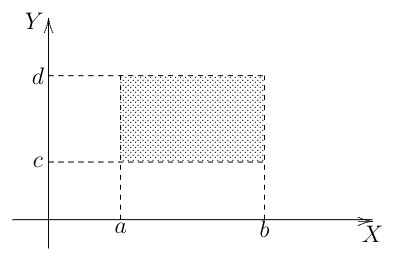
\includegraphics[width=0.5\textwidth]{rectangle2_2_9.png}
    % \caption{Podpis pod obrazkiem}
\end{figure}

Wtedy $\mathbb{B}$ jest baza topologii na plaszczyznie. Ta topologia nazywa sie topologia euklidesowa.

Aby dostrzec, ze $\mathbb{B}$ jest rzeczywiscie baza topologii, zauwazmy ze (i) plaszczyzna jest suma wszystkich takich otwartych prostokatow oraz (ii) przekroj dowolnych dwoch prostokatow jest prostokatem. Przez prostokat rozumiemy tu taki prostokat z bokami rownoleglymi do osi $X$ i $Y$, tak jak na obrazku. Zatem wlasnosci z lematu 2.2.8 zachodza wiec $\mathbb{B}$ jest baza.

\begin{tcolorbox}[colback=white!90!green,colframe=black!35!green,title=2.2.10 Lematokomentarz: Uogolnienie Przykladu 2.2.9]

    Uogolniajac przyklad 2.2.9 mozemy zauwazyc jak polozyc topologie na $\mathbb{R}^{n} = \left\{ \langle x_{1}, x_{2}, \dots, x_{n} \rangle : x_{i} \in \mathbb{R}, i = 1, \dots, n \right\}$, dla dowolnego calkowitego $n > 2$. Przyjmujemy tutaj, ze $\mathbb{B}$ jest kolekcja wszystkich podzbiorow $\left\{ \langle x_{1}, x_{2}, \dots, x_{n} \rangle :a_{i} <  x_{i} < b_{i}, i = 1, \dots, n \right\} \subseteq \mathbb{R}^{n}$ z bokami rownoleglymi do osi ukladu wspolrzednych. Taka kolekcja $\mathbb{B}$ jest baza dla \textbf{topologii euklidesowej} na $\mathbb{R}$.
\end{tcolorbox}

\textbf{Cwiczenia 2.2}

\hrulefill

\begin{enumerate}[align=left] %poczatek zadan 2.2
        \renewcommand{\labelenumi}{\textbf{Cwiczenie 2.2.\arabic{enumi}}}
        
        \myitem W tym cwiczeniu udowodnimy, ze kola(disc)/kula w 2 wymiarach: $\left\{\langle x,y \rangle: x^{2} + y^{2} < 1  \right\}$ jest podzbiorem otwartym ${\mathbb{R}}^2$ oraz kazda otwarte kolo/dysk na plaszczyznie jest zbiorem otwartym.
        \hfill\newline W tym celu:

         \begin{enumerate} 
                \item Niech $\langle a,b \rangle$ bedzie dowolnym punktem w kole $D = \ \left\{\langle x,y \rangle : x^{2} + y^{2} < 1  \right\}$. Polozmy $r = \sqrt{a^{2} + b^{2}}$. Niech $R_{\langle a,b \rangle}$ bedzie otwartym prostokatem z krawedziami w punktach $\langle a \pm \frac{1-r}{8}, b \pm \frac{1-r}{8} \rangle$. Sprawdz ze $R_{\langle a,b \rangle} \subset D$.
                 \item Uzywajac poprzedniego podpunktu (a) udowodnij ze:
                     $$D = \bigcup\limits_{\langle a, b \rangle \in D} R_{\langle a,b \rangle}$$
                 \item Wywnioskuj z (b) ze $D$ jest zbiorem otwartym w ${\mathbb{R}}^{2}$
                 \item Pokaz ze kazde kolo $\left\{ \langle a,b \rangle : (x-a)^{2} + (y-b)^{2}< c^{2}, a,b,c \in \mathbb{R}   \right\}$ jest otwarte w ${\mathbb{R}}^{2}$
        \end{enumerate}

        \myitem W tym cwiczeniu udowodnimy ze kolekcja wszystkich otwartych kol w ${\mathbb{R}}^{2}$ jest baza topologii na $\mathbb{R}^{2}$. Pozniej pokazemy ze jest to indeed topologia euklidesowa. \hfill\newline W tym celu:

        \begin{enumerate}
            \item Niech $D_{1}$ oraz $D_{2}$ bedzie dowolnym otwartym kolem w $\mathbb{R}^{2} z D_{1} \cap D_{2} \neq \emptyset$. Jesli $\langle a, b \rangle$ jest dowolnym punktem w $D_{1} \cap D_{2}$, pokaz ze istnieje otwarte kolo $D_{\langle a,b \rangle}$ z srodekiem w $\langle a,b \rangle$ takie ze $D_{\langle a,b \rangle} \subset D_{1} \cap D_{2}$.
            \item Pokaz ze $$D_{1} \cap D_{2} = \bigcup\limits_{\langle a,b \rangle \in D_{1} \cap D_{2}}D_{\langle a,b \rangle}$$
            \item Uzywajac poprzedniego podpunktu (b) oraz Lematu 2.2.8 udowodnij ze kolekcja wszystkich otwartych kol w $\mathbb{R}^{2}$ jest baza dla topologii na $\mathbb{R}^{2}$.
        \end{enumerate}
        \myitem Niech $\mathbb{B}$ bedzie kolekcja wszystkich otwartych odcinkow $(a,b)$ w $\mathbb{R}$ z a < b, i $a,b \in \mathbb{Q}$. Udowodnij ze $\mathbb{B}$ jest baza dla topologii euklidesowej na $\mathbb{R}$. Porownaj to z Lematem 2.2.1 i Cwiczeniem 2.2.3 gdzie a i b nie byly koniecznie liczbami wymiernymi.
        \myitem \textcolor{red}{Drugi Aksjomat Przeliczalnosci} 
        Mowimy ze przestrzen topologiczna $(X,T)$ spelnia \textcolor{red}{drugi aksjomat przeliczalnosci} albo ze jest \textcolor{red}{drugo przeliczalna? second countable} jesli istnieje baza $\mathbb{B}$ dla $T$, gdzie $\mathbb{B}$ zawiera tylko przeliczalnie wiele zbiorow.

        \begin{enumerate}
            \item Uzywajaz cwiczenia 2.2.3 powyzej, pokaz ze $\mathbb{R}$ spelnia drugi aksjomat przeliczalnosci.
            \item Udowodnij ze przestrzen dyskretna na nieprzeliczalnym zbiorze nie spelnia drugiego aksjomatu przeliczalnosci. Uwaga nie wystarczy ze pokazesz ze jedna konkretna baza jest nieprzeliczalna. Musisz udowodnic ze kazda baza dla tej topologii jest nie przeliczalna.
            \item Udowodnij ze $\mathbb{R}^{n}$ spelnia drugi aksjomat przeliczalnosci dla kazdego n dodatniego, calkowitego.
            \item Niech $(X,T)$ bedzie zbiorem wszystkich liczb calkowitych z skonczenie-domknieta topologia. Czy $(X,T)$ spelnia drugi aksjomat przeliczalnosci?
            
        \end{enumerate}
        \myitem Udowodnij ponizsze stwierdzenia
        \begin{enumerate}
            \item Niech $m,c \in \mathbb{R}$. Wtedy linia $L = \left\{ \langle x,y \rangle: y = mx + c \right\}$ jest domknietym podzbiorem $\mathbb{R}^{2}$
            \item Niech $\mathbb{S}^1$ bedzie kolem jednostkowym, tj. $\mathbb{S}^{1} = \left\{ \langle x,y \rangle \in \mathbb{R}^{2} : x^{2} + y^{2} < 1  \right\}$. Wtedy $\mathbb{S}^{1}$ jest domknietym podzbiorem $\mathbb{R}^2$.
            \item Niech $ \mathbb{S}^n$ bedzie n-sfera jednostkowa, tj. $$\mathbb{S}^{n} = \left\{ \langle x_{1}, x_{2}, \dots, x_{n+1} \in \mathbb{R}^{n+1} : x_{1}^{2} x_{2}^{2} + \dots + x_{n+1}^{2} = 1 \rangle \right\}$$. Pokaz ze $\mathbb{S}^n$ jest zbiorem domknietym w $\mathbb{R}^{n+1}$.
            \item Niech $\mathbb{B}^{n}$ bedzie domknieta n-kula jednostkowa, tj.
                $$\mathbb{B}^{n} = \left\{ \langle x_{1}, x_{2}, \dots, x_{n} \in \mathbb{R}^{n} : x_{1}^{2} x_{2}^{2} + \dots + x_{n+1}^{2} \leq 1 \rangle \right\}$$             
            \item Krzywa $\mathbb{C} = \left\{ \langle x,y \rangle \in \mathbb{R}^{2}:  xy = 1    \right\}$ jest domknieta w $\mathbb{R}^{2}$
            
        \end{enumerate}

        \myitem \textcolor{red}{Iloczyn topologii(product topology)}
        Niech $\mathbb{B}_{1}$ bedzie baza topologii $T_{1}$ na zbiorze $X$ oraz $\mathbb{B}_{2}$ baza dla topolotii $T_{2}$ na zbiorze $Y$. Zbior $X \times Y$ zawierajacy wszystkie mozliwe pary $\langle x, y \rangle$, gdzie $x \in X$ oraz $y \in Y$. Niech $\mathbb{B}$ bedzie kolekcja podzbiorow $X \times Y$ zawierajacych wszystkjie zbiory $B_{1} \times B_{2}$, gdzie $B_{1} \in \mathbb{B}_{1}$ oraz $B_{2} \in \mathbb{B}_{2}$. Udowodnij ze $\mathbb{B}$ jest baza dla topologii na $X \times Y$. Topologia taka nazywa sie \textcolor{red}{topologia produktowa}. Hint: Cwiczenie 2.2.9.
        \myitem Uzywajac Cwiczenia 3 powyzej oraz Cwiczenia 2.1.8, udowodnij ze kazdy zbior otwarty w $\mathbb{R}$ jest $F_{\sigma}$-zbiorem oraz $G_{\delta}$-zbiorem.
        
\end{enumerate}%koniec zadan 2.2
\subsection{Baza dla podanej wczesniej topologii}

Lemat 2.2.8 powiedzial nam pod jakimi warunkami kolekcja $\mathbb{B}$ podzbiorow $X$ jest baza dla \textbf{pewnej} topologii na $X$. Jednakze czasami mamy juz \textbf{ustalona} topologie $T$ na $X$ i chcemy sie dowiedziec czy $\mathbb{B}$ jest baza dla dokladnie tej topologii $T$. Mozemy to owczywiscie sprawdzic z definicji 2.2.2 Bazy topologii, ale lemat 2.3.2 pokazuje nam alternatywna metode.

Spojrzmy najpierw na pewien przyklad:

\textbf{Przyklad 2.3.1}

Niech $\mathbb{B}$ bedzie kolekcja odcinkow jednostronnie domknietych postaci $(a, b]$, $a<b$, gdzie $(a,b] = \left\{ x: x \in \mathbb{R}, a < x \leq b  \right\}$. Wtedy $\mathbb{B}$ jest baza dla topologii na $\mathbb{R}$, poniewaz $\mathbb{R}$ jest suma wszystkich elementow z $\mathbb{B}$ oraz przekroj dowolnych dwoch jednostronnie otwartych odcinkow, jest jednostornnie otwartym odcinkiem. 

\textbf{Jednakze:}

Topologia $T$ ktora ma $\mathbb{B}$ jako swoja baze, \textbf{nie} jest topologia euklidesowa na $\mathbb{R}$.

Dlaczeg? Zauwazmy, ze $(a,b]$ jest zbiorem otwartym w $\mathbb{R}$ z topologia $T$, podczas gdy $(a,b]$ nie jest zbiorem otwartym w $\mathbb{R}$ z topologia euklidesowa. (nie mozemy otoczyc punktu b "odcinkiem otwartym"- dowod cwiczneie 2.1).

Podsumowoujac, $\mathbb{B}$ jest baza dla \textbf{pewnej} topologii ale nie jest baza dla topologii euklidesowej na $\mathbb{R}$.

\begin{tcolorbox}[colback=white!90!green,colframe=black!35!green,title=2.3.2 Lemat Baza topologii podejscie 2?]

    Niech $(X,T)$ bedzie przestrzenia topologiczna. Rodzina $\mathbb{B}$ otwartych podzbiorow $X$ jest baza $T$ wtedy i tylko wtedy kiedy dla dowolnego punktu $x$ nalezacego do dowolnego zbioru otwartego $U$, istnieje zbior $B \in \mathbb{B}$ taki ze $x \in B \subseteq U$.

    Czyli rodzina zbiorow $\mathbb{B}$ jest baza iff dla dowolnego punktu z dowolnego zbioru istnieje zbior bazowy B taki ze $x \in B \subseteq U$
\end{tcolorbox}

\textbf{Dowod:}

Musimy pokazac ze:
\begin{itemize}
    \item jesli $\mathbb{B}$ jest baza $T$ oraz $x \in U \in T$, to istnieje $B \in \mathbb{B}$ takie ze $x \in B \subseteq U$

        oraz
    \item jesli dla kazdego $U \in T$ i $x \in U$ istnieje $B \in \mathbb{B}$ takie ze $x \in B \subseteq U$, wteedy $\mathbb{B}$ jest baza $T$.
\end{itemize}

Zatem:

Zalozmy ze $\mathbb{B}$ jest baza $T$ oraz $x \in U \in T$. Poniewaz $\mathbb{B}$ jest baza $T$, wiec $U$ jest suma otwartych zbiorow z $\mathbb{B}$. To znaczy $U = \bigcup\limits_{j \in J}B_{j}$ dla pewnego zbioru indeksowego $J$ i $B_{j} \in \mathbb{B}$. Ale $x \in U$ implikuje to ze $x \in B_{j}$ dla pewnego $j \in J$. Zatem $x \in B_{j} \subseteq U$, tak jak chcielismy.

Z drugiej strony, zalozmy ze dla kazdego $U \in T$ and kazdego $x\in T$ istnieje $B \in \mathbb{B}$ z $x \in B \subseteq U$. Pokazemy ze kazdy zbior otwarty jest suma elementow z $\mathbb{B}$. Wiec niech $V$ bedzie dowolnym zbiorem otwartym. Wtedy dla kazdeggo $x \in V$, istnieje $B_{x} \in B$ taki ze $x \in B_{x} \subseteq V$. Zauwazmy ze $V = \bigcup\limits_{x \in V}B_{x}$ $\leftarrow$\textbf{UDOWODNIJ TODO}. Zatem $V$ jest suma elementow z $\mathbb{B}$.

\begin{tcolorbox}[colback=white!90!green,colframe=black!35!green,title=2.3.3 Lemat: Baza topologii podejscie 3?]

    Niech $\mathbb{B}$ bedzie baza topologii $T$ na zbiorze $X$. Wtedy podzbior $U$ zbioru $X$ jest otwarty wtedy i tylko wtedy kiedy dla kazdego $x \in U$ istnieje $B \in \mathbb{B}$ takie ze $x \in B \subseteq U$

\end{tcolorbox}

\textbf{Dowod:}

Niech $U$ bedzie dowolnym podzbiorem $X$. Zalozmy ze dla kazdego $x \in U$ istnieje $B_{x} \in \mathbb{B}$ taki ze $x \in B_{x} \subseteq U$. Widac ze $U = \bigcup\limits_{x \in U}B_{x}\leftarrow$\textbf{TUTAJ TROCHE NIE KUMAM ZROB DOWOD I PRZEANALIZUJ} Zatem $U$ jest suma zbiorow otwartych i co za tym idzie $U$ jest zbiorem otwartym. Dowod w druga strone wynika z lematu 2.3.2.

\textbf{Komentarz}

Zauwazmy ze wlasnosc bazy opisana w lemacie 2.3.3 jest dokladnie ta wlasnoscia, ktora uzylismy aby opisac topologie euklidesowa na $\mathbb{R}$. Powiedzielsimy wtedy, ze podzbior $U \subseteq \mathbb{R}$ jest otwarty iff dla kazdego $x \in U$ istnieje $a,b \in \mathbb{R}$ i $a<b$ takie, ze $x \in (a,b) \subseteq U$

\textbf{ATTENZIONE}

Miej na uwadze i pamietaj, o roznicy w lematach 2.2.8 i 2.3.2. W lemacie 2.2.8 podalismy wlasnosci jakie musi miec rodzina $\mathbb{B}$ aby baza dla \textbf{pewnej} topologi, podczas gdy lemat 2.3.2 daje nam wlasnosci jakie musi miec rodzina $\mathbb{B}$ podzbiorow przestrzeni topologicznej $(X,T)$ aby byc baza \textbf{danej} topologii $T$.

\begin{tcolorbox}[colback=white!90!green,colframe=black!35!green,title=2.3.4 Lemat: Bazy dla tej samej topologii]
    Niech $B_{1}$ oraz $B_{2}$ beda bazami dla topologii odpowiednio $T_{1}$ oraz $T_{2}$, na niepustym zbiorze $X$. Wtedy $T_{1} = T_{2}$ wtedy i tylko wtedy kiedy:
    \begin{enumerate}[label=(\alph*)]
        \item dla kazdego $B \in B_{1}$ i kazdego $x \in B$, istnieje $B^{\prime} \in B_{2}$ takie ze $x \in B^{\prime} \subseteq B$, oraz
        \item dla kazdego $B \in B_{2}$ i kazdego $x \in B$, istnieje $B^{\prime} \in B_{1}$ takie ze $x \in B^{\prime} \subseteq B$
    \end{enumerate}
\end{tcolorbox}

\textbf{Dowod:}

Pokazemy ze $B_{1}$ oraz $B_{2}$ sa bazami dla tej samej topologii iff (a) oraz (b) zachodza. Najpierw zalozymy ze one sa bazami dla tej samej topologii, tzn $T_{1} = T_{2}$ i pokazemy za (a) i (b) zachodza. Nastepnie zalozymy ze (a) i (b) zachodza i pokazemy ze $T_{1} = T_{2}$.

Zatem:

Najpierw zalozmy ze $T_{1} = T_{2}$. Wtedy (a) i (b) sa konsekwencja lematu 2.3.2

Z drugiej strony, zalozmy, ze $B_{1}$ oraz $B_{2}$ spelniaja warunki (a) oraz (b). Na mocy lematu 2.3.2, (a) implikuje to, ze kazde $B \in B_{1}$ jest otwarte w $(X,T_{2})$; to znaczy $B_{1} \subseteq T_{2}$. Poniewaz kazdy element $T_{1}$ ja suma elementow z $T_{2}$, implikuje to $T_{1} \subseteq T_{2}$. Analogicznie (b) pociaga za soba $T_{2} \subseteq T_{1}$. Czyli $T_{1} = T_{2}$, tak jak chcielismy.

Spojrzmy teraz na przyklady.

\textbf{2.3.5 Przyklad}

Pokaz,ze zbior $\mathbb{B}$ skladajacy sie z wszyskich "otwartych trojkatow rownobocznych" z podstawa rownolegla do osi X, jest baza dla topologi euklidesowej na $R^{2}$.(Otwarty, czyli bez brzegu).

\textbf{Dowod przez obrazki i tlumeczenie. TODO FORMALNY DOWOD!!!!!}

Musimy pokazac ze $\mathbb{B}$ jest baza dla topologii euklidesowej. Zastosujemy lemat 2.3.4 ale najpierw musimy pokazac, ze $\mathbb{B}$ jest baza dla \textbf{jakiejs} topologii na $\mathbb{R}^{2}$ 

Aby to zrobic, pokazemy ze $\mathbb{B}$ spelnia warunki z lematu 2.2.8

\begin{center}
    \begin{minipage}[h]{0.8\textwidth}
        \centering
        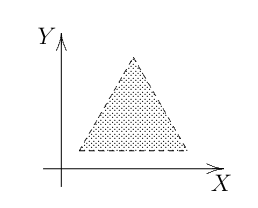
\includegraphics[width=0.5\textwidth]{trojkat1.png}
         %\caption{Podpis pod obrazkiem}
    \end{minipage}
\end{center}

Pierwsza rzecza ktora nalezy zauwazyc jest to, ze $\mathbb{B}$ jest baza dla jakiejs topologii poniewaz spelnia warunki z lematu 2.2.8. Aby to zauwazyc, spojrz ze $\mathbb{R}^{2}$ jest rowne sumie wszystkich otwartych trojkatow rownobocznych z podstawa rownolegla do osi X oraz ze przeciecie dwoch dowolnych trojkatow jest kolejnym trojkatem. ?

Nastepnie pokazemy ze warunki (a) oraz (b) z lematu 2.3.4 sa spelnione.

Najpierw sprawdzimy warunek (a). Niech R bedzie otwartym prostokatem z bokami rownoleglymi do osi ukladu oraz x dowolnym punktem w R. Pokazemy ze istnieje otwarty trojkart rownoboczny T z podstawa rownolegla do osi X taki ze $x \in T \subseteq R$. Na obrazku latwo to zauwazyc.

\begin{center}
    \begin{minipage}[h]{0.8\textwidth}
        \centering
        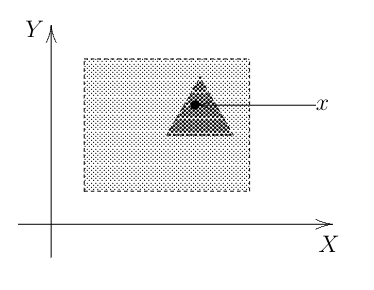
\includegraphics[width=0.5\textwidth]{trojkat2.png}
        %\caption{Podpis pod obrazkiem}
    \end{minipage}
\end{center}

W koncu sprawdzamy warunek (b) z lematu 2.3.4. Niech $T^{\prime}$ bedzie otwartym trojkatem rownobocznym z podstawa rownolegla do osi X oraz niech y bedzie dowolnym punktem w $T^{\prime}$. Wtedy istnieje otwarty prostokat $R^{\prime}$ taki ze $y \in R^{\prime} \subseteq T^{\prime}$. Ponownie na obrazku jest latwo to dostrzec.

\begin{center}
    \begin{minipage}[h]{0.8\textwidth}
        \centering
        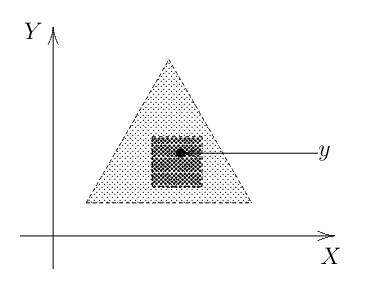
\includegraphics[width=0.5\textwidth]{trojkat3.png}
         %\caption{Podpis pod obrazkiem}
    \end{minipage}
\end{center}


Zatem warunkiz lematu 2.3.4 sa spelnione. Zatem $\mathbb{B}$ jest rzeczywiscie baza dla topologi euklidesowej na $R^{2}$.

\vspace{1cm}

W przykladzie 2.2.9 zdefiniowalismy sobie baze dla topologii euklidesowej jako kolekcje "otwartych prostokatow" (z bokami rownoleglymi do osi ukladu). Przyklad 2.3.5 pokazal nam ze "otwarte prostoakaty" moga byc wymienione przez "otwarte trojkaty rownoboczne"(z podstawa rownolegla do osi X) bez potrzeby zmiany topologii. W cwiczeniu 2.3 1 zobaczymy ze warunki w nawiasach(rownoleglosc) moga zostac porzucone bez potrzeby zmiany topologii. Co wiecej "otwarte prostokaty" moga zostac wymienione na "otwarte kola".

\textbf{Cwiczenia 2.3}

\hrulefill

\begin{enumerate}[align=left] %poczatek zadan 2.3
        \renewcommand{\labelenumi}{\textbf{Cwiczenie 2.3.\arabic{enumi}}}
        \myitem Okresl czy podane kolekcje sa baza dla topologii euklidesowej na $\mathbb{R}^{2}$
        
        \begin{enumerate}
            \item kolekcja wszystkich "otwartych kwadratow" z bokami rownoleglymi do osi ukladu
            \item kolekcja wszystkich otawrtych kol(disc)
            \item kolekcja wszystkich otwartych kwadratow
            \item kolekcja wszystkich otwartych prostokatow
            \item kolekcja wszystkich otwartych trojkatow
          
        \end{enumerate}

        \myitem
            \begin{enumerate}
                \item Niech $\mathbb{B}$ bedzie baza dla topologii $T$ na niepustym zbiorze $X$. Jesli $\mathbb{B}_{1}$ jest kolekcja podzbiorow $X$, taka ze $\mathbb{B} \subseteq \mathbb{B}_{1} \subseteq T$. Udowodnij ze $\mathbb{B}_{1}$ jest takze baza dla $T$.
                \item Wywnioskuj z (a), ze istnieje nieprzeliczalnie liczba roznych baz dla topologii euklidesowej na $\mathbb{R}$
            \end{enumerate}
         \myitem Niech $\mathbb{B} = \left\{ (a,b]: a,b \in \mathbb{R}, a<b \right\}$. Tak jak widzielismy w Cwiczeniu 2.3.1, $\mathbb{B}$ jest baza dla topologii $T$ na $\mathbb{R}$ oraz $T$ nie jest topologia euklidesowa na $\mathbb{R}$. Niemniej, pokaz ze kazdy odcinek otwarty $(a,b)$ jest otwarty w $(\mathbb{R}, T)$.
         \myitem Niech $C[0,1]$ oznacza zbior wszystkich funkcji rzeczywistych ciaglych na odcinku $[0,1]$.
         \begin{enumerate}
             \item Pokaz ze kolekcja $\mathbb{M}$, gdzie $\mathbb{M} = \left\{ M(f, \epsilon): f \in C[0,1], \epsilon \in \mathbb{R}^{+}    \right\}$ oraz $M(f, \epsilon) =  \left\{g: g \in C[0,1] \land \int_{{0}}^{{1}} {|f(x)-g(x)|} \: d{x} {< \epsilon} \right\} $ jest baza dla topologii $T_{1}$ na $C[0,1]$.
             \item Pokaz ze kolekcja $\mathbb{U} = \left\{U(f,\epsilon); f\in C[0,1] \land \epsilon \in \mathbb{R}^{+} \right\}$ oraz $U(f, \epsilon) = \left\{g: g \in C[0,1] \land sup_{x\in [0,1]} |f(x) - g(x)| < \epsilon  \right\}$ jest baza dla topologii $T_{2}$ na $C[0,1]$.
             \item Udowodnij ze $T_{1} \neq T_{2}$
         \end{enumerate}
         \myitem \textcolor{red}{Podbaza dla topologii(Subbasis for a topology)}
         Niech $(X,T)$ bedzie przestrzenia topologiczna. Mowimy ze niepusta kolekcja $\mathbb{S}$ otwartych podzbiorow $X$ jest \textcolor{red}{podbaza(subbasis)} $T$ jesli kolekcja wszystkich skonczonych przekrojow elementow $ \mathbb{S}$ formuje nam baze dla $T$.
         \begin{enumerate}
             \item Udowodnij ze kolekcja wszystkich wszystkich otwartyc odcinkow postaci $(a, \infty)$ lub $(-\infty, b)$ jest podbaza(subbasis) topologii euklidesowej na $\mathbb{R}$.
             \item Udowodnij ze $\mathbb{S} = \left\{ \left\{ a \right\}, \left\{ a,c,d \right\}, \left\{ b,c,d,e,f \right\}  \right\}$ jest podbaza dla topologii $T_{1}$ z przykladu 1.1.2
             
         \end{enumerate}

         \myitem Niech $\mathbb{S}$ bedzie podbaza dla topologii $T$ na $\mathbb{R}$. Zalozmy, ze wszystkie domkniete odcinki $[a,b]$, a<b sa w $\mathbb{S}$. Udowodnij ze $T$ jest topologia dyskretna.
        
        \myitem Niech $X$ bedzie zbiorem z conajmniej dwoma elementami oraz $\mathbb{S}$ kolekcja wszystkich zbiorow postaci $X \setminus \left\{ x\right\}$, $x\in X$. Udowodnij ze $\mathbb{S}$ jest podbaza dla skonczenie-domknietej topologii na $X$.
        \myitem Niech $X$ bedzie dowolnym zbiorem nieskonczonym oraz $T$ topologia dyskretna na $X$. Znajdz podbaze $\mathbb{S}$ dla $T$, taka ze $\mathbb{S}$ nie zawiera zadnego singletonu.
        \myitem Niech $\mathbb{S}$ bedzie kolekcja wszystkich lini prostych na plaszczyznie $\mathbb{R}^{2}$. Jesli $\mathbb{S}$ jest podbaza dla topologii $T$ na $\mathbb{E}^{2}$, to jaka(czym/co to za topologia) jest topologia?
        \myitem Niech $\mathbb{S}$ bedzie kolekcja wszystkich lini prostych, ktore sa rownolegle do osi $X$. Jesli $\mathbb{S}$ jest podbaza topologii $T$ na $\mathbb{R}^{2}$ to opisz zbiory otwarte przestrzeni topologicznej $(\mathbb{R}^{2}, T)$.
        \myitem Niech $\mathbb{S}$ bedzie kolekcja wszystkich kol na plaszczyznie. Jesli $\mathbb{S}$ jest podbaza dla topologii $T$ na $\mathbb{R}^{2}$, to opisz zbiory otwarte w $(\mathbb{R}^{2}, T)$
        \myitem Niech $\mathbb{S}$ bedzie kolekcja wszystkich kol na plaszczyznie ktore maja srodek polozony na osi $X$. Jesli $\mathbb{S}$ jest podbaza dla topologii $T$ na $\mathbb{R}^{2}$, to opisz zbiory otwarte w $(\mathbb{R}^{2}, T)$.

\end{enumerate}%koniec zadan 2.3

\section{Punkty skupienia(ang Limit Points)}

\subsection{Punkty skupienia i domkniecie}

Majac przestrzen topologiczna $(X.T)$, zwykle sie przyjelo, ze na elementy zbioru $X$ mowi sie, ze sa \textbf{punktami}.

\begin{tcolorbox}[colback=white!90!red,colframe=black!35!red,title=3.1.1 Definicja: Punkt skupienia(limit point/accumulation point/clusterpoint)]

    Niech $A$ bedzie podzbiorem przestrzeni topologicznej $(X,T)$. Punkt  $x\in X$ jest punktem skupienia(ang. limit point/accumulation point/cluster point) zbioru $A$ jesli kazdy zbior otwarty $U$, zawierajacy $x$, zawiera tez punkt nalezacy do $A$, ale rozny od $x$.

\end{tcolorbox}

\textbf{3.1.2 Przyklad}

Rozwazmy przestrzen topologiczna $(X,T)$ gdzie $X = \left\{ a,b,c,d,e, \right\}$ oraz topologia $T = \left\{X, \emptyset, \left\{ a \right\}, \left\{ c, d \right\}, \left\{ a,c,d \right\}, \left\{ b,c,d,e \right\}  \right\}$ oraz $A = \left\{ a,b,c \right\}$. Wtedy b, d oraz e sa punktami skupienia zbioru $A$ ale a i c nie sa punktami skupienia zbioru $A$.

\textbf{Dowod}

Zbior $\left\{ a \right\}$ jest otwarty i nie zawiera zadnego innego punktu z $A$. Zatem a nie jest punktem skupienia.

Jedynym zbiorem otwartym zawierajacym b jest $X$ oraz $\left\{ b,c,d,e \right\}$ i oba te zbiory zawieraja punkt nalezacy do $A$ ale inny od $x$. Zatem b jest punktem skupienia zbioru $A$.

Punkt d jest punktem skupienia zbioru $A$, pomimo tego ze nie nalezy do $A$. Jest tak poniewaz kazdy zbior otwarty zawierajacy d, zawiera punkt z $A$ inny od d. Analogicznie jest z punktem e, takze jest on punktem skupienia zbioru $A$ nawet pomimo tego, ze nie nalezy do $A$.


\textbf{3.1.3 Przyklad}

Niech $(X, T)$ bedzie przestrzenia dyskretna oraz $A$ podzbiorem $X$. Wtedy $A$ nie ma punktow skupienia, gdyz dla kazdego $x \in X$, $\left\{ x \right\}$ jest zbiorem otwartym i nie zaweira on punktu z $A$ innego niz x.

\textbf{3.1.4 Przyklad}

Rozwazmy podzbior $A = [a,b) \subseteq \mathbb{R}$. Latwo udowodnic ze kazdy element $[a,b)$ jest punktem skupienia $A$.$\leftarrow \text{UDOWODNIJ!!!!} $Punkt b jest takze punktem skupienia $A$  

\textbf{3.1.5 Przyklad}
Niech $(X,T)$ bedzie przestrzenia niedyskretna oraz $A$ podzbiorem $X$ z conajmniej dwoma elementami. Latwo pokazac(\textbf{UDOWDNIJ!!!!)}, ze kazdy punkt $X$ ma punkt skupienia w $A$ (\textbf{TODO} UDOWODNIJ I POKAZ DLACZEGO SA YWMAGANE CONAJMNIEJ 2 ELEMENTY!!!!)

Ponizszy lematokometarz dostarcza pozytecznego narzedzia do sprawdzania czy zbior jest domkniety czy nie.

\begin{tcolorbox}[colback=white!90!green,colframe=black!35!green,title=3.1.6 Lematokomentarz: Warunek na domknietosc A]

    Niech A bedzie podzbiorem przestrzeni topologicznej $(X,T)$. Wtedy $A$ jest domkniety w $(X,T)$ wtedy i tylko wtedy kiedy $A$ zawiera wszystkie punkty skupienia.

\end{tcolorbox}

\textbf{Dowod}

$(\rightarrow)$

Zalozmy, ze $A$ jest domkniety w $(X,T)$. Zalozmy nie wprosc, ze $p$ jest punktem skupienia zbioru $A$, takim, ze $p \in X\setminus A$. Wtedy $X\setminus A$ jest zbiorem otwartym zawierajacym punkt skupienia $p$ zbioru $A$. Zatem $X\setminus A$ zawieta element z $A$. To jest oczywiscie falsz, mamy sprzecznosc z zalozeniem. Zatem kazdy punkt skupienia zbioru $A$ musi znajdowac sie w $A$.

$(\leftarrow)$

Zalozmy, ze $A$ zawiera wszystkie punkty skupienia. Zatem dla kazdego $z \in X\setminus A$, istnieje zbior otwarty $U_{z}$, $z \in U_{z}$ taki ze, $U_{z} \cap A = \emptyset$; czyli $U_{z} \subseteq X\setminus A$. Zatem $X\setminus A = \bigcup\limits_{z \in X\setminus A}U_{z}$ (\textbf{UDOWODNIJ!!!!!!!!!}). Zatem $X\setminus A$ jest suma zbiorow otwartycz wiec jest otwarta. Zatem jej dopelnienie, $A$, jest domkniete. 

\textbf{3.1.7 Przyklad}

Jako zastosowanie lematokomentarzu 3.1.6 mamy nastepujace wnioski:
\begin{itemize}
    \item zbior [a,b) nie jest domkniety w $\mathbb{R}$, bo b jest punktem skupienia i $b \not\in [a,b)$;
    \item zbior $[a,b]$ jest domkniety w $\mathbb{R}$, poniewaz wszystkie punkty skupienia $[a,b]$(zauwazmy ze sa to wszystkie punktu [a,b]) sa w $[a,b]$
    \item $(a,b)$ nie jest zbiorem domknietym w $\mathbb{R}$, poniewaz nie zawiera punktu skupienia $a$
    \item $[a, \infty)$ nie jest zbiorem domknietym w $\mathbb{R}$  
\end{itemize}

\begin{tcolorbox}[colback=white!90!green,colframe=black!35!green,title=3.1.8 Lematokomentarz: domknietosc  $A \cup A^{\prime}$]

    Niech $A$ bedzie podzbiorem przestrzeni topologicznej $(X,T)$ oraz $A^{\prime}$ zbiorem wszystkich punktow skupienia zbioru $A$. Wtedy $A \cup A^{\prime}$ jest zbiorem domknietym.

\end{tcolorbox}

\textbf{Dowod}

Z Lematu 3.1.6 wystarczy pokazac, ze zbior $A \cup A^{\prime}$ zawiera wszyskie \textbf{swoje} punkty skupienia lub rownowaznie, ze zaden element zbioru $X \setminus A\cup A^{\prime}$ nie jest punktem skupienia zbioru $A\cup A^{\prime}$

Niech $p \in X \setminus A \cup A^{\prime}$. Poniewaz $p \notin A^{\prime}$, to istnieje zbior otwarty $U$ zawierajacy $p$ taki ze $U \cap A = \left\{ p \right\}$ albo $\emptyset$. Ale $p\notin A$ wiec $U\cap A = \emptyset$. Twierdzimy tez, ze $U \cap A^{\prime} = \emptyset$. Jesli tak nie jest, to $x \in U$, wtedy $U$ jako zbior otwarty i $U\cap A = \emptyset$ daje $x\notin A^{\prime}$. Zatem $U\cap A^{\prime} = \emptyset$. Zatem $U \cap (A\cup A^{\prime}) = \emptyset$ oraz $p\in U$. Czyli $p$ nie jest punktem skupienia $A\cup A^{\prime}$, co za tym idzie, $A\cup A^{\prime}$ domkniety.

\begin{tcolorbox}[colback=white!90!red,colframe=black!35!red,title=3.1.9 Definicja: Domkniecie zbioru A(closure of A)]

    Niech A bedzie podzbiorem przestrzeni topologicznej $(X,T)$. Wtedy zbior $A\cup A^{\prime}$ zawierajacy A oraz wszystkie jego punkty skupienia jest nazywany \textbf{domknieciem zbioru A(closure of A)} i ma swoje oznaczenie, mianowicie: $\overline{A}$

\end{tcolorbox}

\textbf{3.1.10 Uwaga}

Jest jasne z Lematu 3.1.8 ze $\overline{A}$ jest zbiorem domknietym. Lemat 3.1.6 oraz cwiczenie 3.1.5(i) mowia, ze kazdy zbior domkniety zawierajacy A musi takze zawierac zbior $A^{\prime}$. Zatem $A \cup A^{\prime} = \overline{A}$ jest najmniejszym domknietym zbiorem zawierajacym $A$. Co za tym idzie $\overline{A}$ jest przekrojem wszystkich zbiorow domknietych zawierajacych $A$.

\textbf{3.1.11 Przyklad}

Niech $X = \left\{ a,b,c,d,e \right\}$ oraz $T = \left\{ X, \emptyset, \left\{ a \right\}, \left\{ c,d \right\}, \left\{ a,c,d \right\}, \left\{ b,c,d,e \right\}  \right\}$. Pokaz, ze $\overline{\left\{b\right\}} = \left\{ b,e \right\}, \overline{\left\{a,c\right\}} = X, \overline{\left\{b,d\right\}} = \left\{ b,c,d,e \right\} $

\textbf{Komentarz}

Aby znalezc domkniecie danego zbioru, powinnismy znalezc najpierw wszystkie zbiory domkniete zawierajace ten zbior oraz wybrac najmniejszy. Zatem zaczniemy od wypisania wszystkich zbiorow domknietych- sa to po prostu dopelnienia otwartych zbiorow.

\textbf{Dowod}

Zbiorami domknietymi sa $\emptyset, X, \left\{ b,c,d,e \right\}, \left\{ a,b,e \right\}, \left\{ b, e \right\}, \left\{ a \right\}$. Zatem najmniejszym zbiorem zawierajacym $\left\{ b \right\}$ jest $\left\{ b,e \right\}$; zatem  $\overline{\left\{b\right\}} = \left\{ b,e \right\}$. Analogicznie $\overline{\left\{a,c\right\}} = X$ oraz $\overline{\left\{b,d\right\}} = \left\{ b,c,d,e \right\}$ 

\textbf{3.1.12 Przyklad}

Udowodnic ze $\overline{\mathbb{Q}} = \mathbb{R}$.

\textbf{Dowod}

Zalozmy ze $\overline{\mathbb{Q}} \neq \mathbb{R}$. Wtedy istnieje $x \in \mathbb{R} \setminus \overline{\mathbb{Q}}$. Poniewaz $\mathbb{R} \setminus \overline{\mathbb{Q}}$ jest otwarty w $\mathbb{R}$ , zatem istnieja a<b takie ze $x\in (a,b) \subseteq \mathbb{R}\setminus \overline{\mathbb{Q}}$. Ale w kazdym odcinku $(a,b)$
istnieje liczba wymierna q; to znaczy $q \in (a,b)$. Zatem $q \in \mathbb{R} \setminus \overline{\mathbb{Q}}$ co za tym idzie, $q\in \mathbb{R}\setminus \\mathbb{Q}$. Otrzymalismy sprzecznosc, bo $q \in \mathbb{Q}$. Zatem $\overline{\mathbb{Q}} = \mathbb{R}$

\begin{tcolorbox}[colback=white!90!red,colframe=black!35!red,title=3.1.13 Definicja: Gestosc]

    Niech $A$ bedzie podzbiorem przestrzeni topologicznej $(X,T)$. Mowimy, ze $A$ jest \textbf{gesty} w $X$ lub \textbf{wszedzie gesty} w $X$ jesli $\overline{A} = X$

\end{tcolorbox}

Zatem, korzystajac z powyzszej definicji, mozemy przeformulowac wniosek z przykladu 3.1.12: zbior $\mathbb{Q}$ jest gestym podzbiorem $\mathbb{R}$.

\textbf{3.1.14 Przyklad}

Niech $(X,T)$ bedzie przestrzenia dyskretna. Wtedy kazdy podzbior $X$ jest domkniety(bo jego dopelnienie jest otwarte). Zatem jedynym gestym podzbiorem $X$ jest $X$, bo kazdy podzbior $X$ jest swoim wlasnym domknieciem.


\begin{tcolorbox}[colback=white!90!green,colframe=black!35!green,title=3.1.15 Lematokomentarz: Gesty zbior A przecina niepusto wszystkie zbiory otwarte]

Niech $A$ bedzie podzbiorem przestrzeni topologicznej $(X,T)$. Wtedy $A$ jest gesty w $X$ wtedy i tylko wtedy kiedy kazdy nie pusty zbior otwarty w $X$ przecina $A$ nie pusto. To znaczy jesli $U \in T$ oraz $U \neq \emptyset$ to $A \cap U \neq \emptyset$

\end{tcolorbox}

\textbf{Dowod}

$(\leftarrow)$

Zalozmy, ze kazdy niepusty zbior otwarty przecina sie z $A$ niepusto. Jesli $A=X$, to ofc $A$ jest gesty w $X$. Jesli $A \neq X$, to niech $x \in X\setminus A$. Jesli $U \in T$ oraz $x \in U$ wtedy $U \cap A \neq \emptyset$. Zatem x jest punktem skupienia zbioru A. Poniewaz x byl dowolnym punktem w $X\setminus A$, to kazdy punkt zbioru $X\setminus A$ jest punktem skupienia zbioru $A$. Zatem $X\setminus A \subseteq A^{\prime}$ i z definicji 3.1.9 $\overline{A} = A^{\prime} \cup A = X$; czyli A jest gesty w X.

$(\rightarrow)$

Zalozmy ze A jest gesty w X. Niech $U$ bedzie dowolnym niepustym zbiorem otwartym w X. Zalozmy ze $U\cap A = \emptyset$. Wtedy jesli $x\in U$ to $x \not\in A$ i x nie jest punktem skupienia zbioru $A$, bo $U$ jest zbiorem otwartym zawierajacym x, ale nic poza tym x ze zbioru $A$. To jest sprzecznosc, bo $A$ jest gesty w $X$, czyli kazdy element $X\setminus A$ jest punktem skupienia zbioru $A$. Zatem nasze zalozenie jest falszywe i $U\cap A \neq \emptyset$, tak jak chcielismy.

\textbf{Cwiczenia 3.1}

\hrulefill

\begin{enumerate}[align=left] %poczatek zadan 3.1
        \renewcommand{\labelenumi}{\textbf{Cwiczenie 3.1.\arabic{enumi}}}

        \myitem 
        \begin{enumerate}
            \item W przykladzie 3.1.2, znajdz wszystki punkty skupienia nastepujacych zbiorow:
                \begin{enumerate}
                    \item $\left\{ a \right\}$
                    \item $\left\{ b,c \right\}$
                    \item $\left\{ a,c,d \right\}$
                    \item $\left\{ b,d,e \right\}$
                \end{enumerate}
            \item Znajdz domkniecia(closure) powyzszych zbiorow
            \item Znajdz domkniecia powyzszych zbiorow ale uzywajac metody z przykladu 3.2.11
        \end{enumerate}
        \myitem Niech $(\mathbb{Z}, T)$ bedzie przestrzenia z skonczenie-domknieta topologia. Wypisz zbior punktow skupienia ponizszych zbiorow:
        \begin{enumerate}
            \item $A = \left\{1,2,\dots,10  \right\}$
            \item Zbior $E$, zawierajacy wszystkie liczby parzyste.
        \end{enumerate}

        \myitem Znajdz wszystkie punkty skupienia odcinka otwartego $(a,b)$ w $\mathbb{R}$, a<b.

        \myitem 
        \begin{enumerate}
            \item Jakie jest domkniecie(closure) w $\mathbb{R}$ kazdego z ponizszych zbiorow.
                \begin{enumerate}
                    \item $\left\{ 1, \frac{1}{2}, \frac{1}{3}, \dots, \frac{1}{n} , \dots \right\}$
                    \item zbior liczb calkowitych $\mathbb{Z}$
                    \item zbior liczb niewymiernych $\mathbb{P}$
                \end{enumerate}
            \item Niech $S$ bedzie niepustym podzbiorem $\mathbb{R}$ oraz $a \in \mathbb{R}$. Udowodnij ze $a \in \overline{S}$ wtedy i tylko wtedy kiedy dla kazdego $n \in \mathbb{N}^{+}$, istnieje ciag $x_{n} \in S$, taka ze $|x_{n}-a| < \frac{1}{n}$.  
        \end{enumerate}

        \myitem
        Niech $S$ oraz $T$ beda niepustymi podzbiorami przestrzeni topologicznej $(X,T)$ oraz $S \subseteq T$
        \begin{enumerate}
            \item Sprawdz ze jesli p jest punktem skupienia zbioru $S$ to p jest takze punktem skupienia zbioru $T$
            \item Wywnioskuj z poprzedniego punktu ze $\overline{S} \subseteq \overline{T}$
            \item Pokaz tez, ze jesli $S$ jest gesty w $X$ to $T$ jest gesty w $X$.
            \item Uzywajac poprzedniego podpunktu pokaz ze $\mathbb{R}$ ma nieprzeliczalnie wiele roznych gestych podzbiorow.
            \item Ponownie uzywajac trzeciego podpunktu. Udowodnij ze $\mathbb{R}$ ma nieprzeliczalnie wiele roznych przeliczalnych gestych podzbiorow oraz $2^{\mathfrak{c}}$ roznych nieprzeliczalnych gestych podzbiorow. To jest z gwiazdka.
            
        \end{enumerate}
        \myitem Niech $A$ oraz $B$ beda podzbiorami przesetrzeni $\mathbb{R}$ z topologia euklidesowa. Rozwazmy 4 zbiory;
        \begin{enumerate}[label=(\roman*)]
            \item $A \cap \overline{B}$
            \item $\overline{A} \cap B$
            \item $\overline{A} \cap \overline{B}$
            \item $\overline{A\cap B}$
        \end{enumerate}
        
        Udowodnij ponizsze stwierdzenia:
        \begin{enumerate}
            \item Jesli $A = \mathbb{Q}$ oraz $B = \mathbb{R} \setminus \mathbb{Q}$ to udowodnij ze powyzsze zbiory sa parami rozne.
            \item Jesli $A$ i $B$ sa otwartymi odcinkami w $\mathbb{R}$ to udowodnij ze conajmniej dwa z powyzszych zbiorow sa rowne.
            \item Wskaz dwa otwarte podzbiory $\mathbb{R}$, $A$ i $B$ takie ze powyzsza czworka zbiorow jest parami rozna.
        \end{enumerate}

\end{enumerate}%koniec zadan 3.1


\subsection{Sasiedztwo/otoczenie (ang Neighbourhoods)}

\begin{tcolorbox}[colback=white!90!red,colframe=black!35!red,title=3.2.1 Definicja: Otoczenie/sasiedztwo]

Niech $(X,T)$ bedzie przestrzenia topologiczna, $N \subseteq X$ oraz punkt $p\in N$. Mowimy, ze $N$ jest \textbf{otoczeniem(neighbourhood)} punktu p, jesli istnieje zbior otwarty $U$, taki ze $p\in U \subseteq N$

\end{tcolorbox}

\textbf{3.2.2 Przyklad}

Domkniety odcinek $[0,1]$ w $\mathbb{R}$ jest otoczneiem punktu $\frac{1}{2} \in (\frac{1}{4}, \frac{3}{4}) \subseteq [0,1]$.

\textbf{3.2.3 Przyklad}

Odcinek jednostronnie domkniety $(0,1]$ w $\mathbb{R}$ jest otoczeniem punktu $\frac{1}{4}$, bo $\frac{1}{4} \in (0, \frac{1}{2}) \subseteq (0,1]$. Ale $(0,1]$ nie jest otoczeniem punktu 1.\textbf{UDOWODNIJ TO TODO} 

\textbf{3.2.4 Przyklad}

Jesli $(X,T)$ jest dowolna przestrzenia topologiczna oraz $U \in T$, wtedy z definicji 3.2.1(definicja otoczenia), wiadomo, ze $U$ jest oroczeniem dowolnego puntku $p\in U$. Zatem, na przyklad, kazdy otwarty odcinek $(a,b)$ w $\mathbb{R}$ jest otoczeniem kazdego punktu, ktory w nim jest.

\textbf{3.2.5 Przyklad}

Niech $(X,T)$ bedzie przestrzenia topologiczna oraz $N$ otoczeniem punktu $p$. Jesli $S$ jest dowolnym podzbiorem $X$, takim ze $N \subseteq S$ to $S$ jest otoczeniem punktu $p$.

\begin{tcolorbox}[colback=white!90!green,colframe=black!35!green,title=3.2.6 Lematokomentarz: Punkt skupienia a otoczenie.]
    Niech $A$ bedzie podzbiorem przestrzeni topologicznej $(X,T)$. Punkt $x\in X$ jest punktem skupienia zbioru $A$ wtedy i tylko wtedy kiedy dowolne otoczenie punktu $x$ zawiera w sobie punkt ze zbioru $A$ inny od $x$ (Czy taki otoczenie punktu x, nie zaweireajace punktu x, to nie jest sasiedztwo? Sprwadz)

\end{tcolorbox}

\textbf{Dowod- Jest prosty i zostawiony dla czytelnika(czyli mnie) TODO}

\begin{tcolorbox}[colback=white!90!cyan,colframe=black!35!cyan,title=3.2.7 Wniosek: Otoczenie i domknietosc zbioru A]

    Niech $A$ bedzie podzbiorem przestrzeni topologicznej $(X,T)$. Wtedy zbior $A$ jest domkniety wtedy i tylko wtedy kiedy dla kazdego $x \in X\setminus A$ istnieje otoczenie $N$ punktu $x$ takie ze $N \subseteq X\setminus A$

\end{tcolorbox}

\begin{tcolorbox}[colback=white!90!cyan,colframe=black!35!cyan,title=3.2.8 Wniosek: Otoczenie i otwartosc zbioru A]

    Niech $U$ bedzie podzbiorem przestrzeni topologicznej $(X,T)$. Wtedy $U\in T$ wtedy i tylko wtedy, kiedy dla kazdego $x\in U$ istnieje otoczenie $N$ punktu $x$, takie ze $N\subseteq U$.

\end{tcolorbox}

\begin{tcolorbox}[colback=white!90!cyan,colframe=black!35!cyan,title=3.2.9 Wniosek: Otoczenie i otwartosc zbioru A: v2]
    Niech $U$ bedzie podzbiorem przestrzeni topologicznej $(X,T)$. Wtedy $U\in T$ wtedy i tylko wtedy, kiedy dla kazdego $x\in U$ istnieje $V \in T$ takie ze $x\in V \subseteq U.$

\end{tcolorbox}



\textbf{Cwiczenia 3.2}

\hrulefill

\begin{enumerate}[align=left] %poczatek zadan 3.2
        \renewcommand{\labelenumi}{\textbf{Cwiczenie 3.2.\arabic{enumi}}}
        \myitem Niech A bedzie podzbiorem przestrzeni topologicznej $(X,T)$. Udowodnij, ze $A$ jest gety w $X$ wtedy i tylko wtedy kazde otoczenie kazdego punktu w $X\setminus A$ przecina sie z $A$ nietrywialnie(?czylijak)
        \myitem Rozwiaz:
        \begin{enumerate}[label=(\roman*)]
            \item Niech $A$ i $B$ beda pozbiorami przestrzeni topologicznej $(X,T)$. Udowodnij dokladnie i uwaznie ze:
                $$\overline{A\cap B} \subseteq \overline{A} \cap \overline{B}$$
            \item Skonstruuj przyklad w ktorym 
            $$\overline{A\cap B} \neq \overline{A} \cap \overline{B}$$
        \end{enumerate}
        \myitem Niech $(X,T)$ bedzie przestrzenia topologiczna. Udowodnij ze $T$ jest skonczenie-domknieta topologia na $X$ wtedy i tylko wtedy kiedy:
        \begin{enumerate}[label=(\roman*)]
            \item $(X,T)$ is $T_{1}$-przestrzenia
            \item kazdy nieskonczony podzbior $X$ jest gesty w $X$
        \end{enumerate}
        \myitem \textcolor{red}{Przestrzenie rozdzielne/oddzielne(and. Separable spaces)}
        Mowimy ze przestrzen topologiczna $(X,T)$ jest \textcolor{red}{rozdzielna/oddzielna(separable)} jesli zawiera gesty podzbior ktory jest przeliczalny. Rozstrzygnij ktore z ponizszych przestrzeni sa rozdzielne:
        \begin{enumerate}[label=(\roman*)]
            \item Zbior $\mathbb{R}$ ze zwykla topologia(euklidesowa?)
            \item Przeliczalny zbior z topologia dyskretna
            \item Przeliczalny zbior z skonczenie-domknieta topologia
            \item $(X,T)$ gdzie $X$ jest skonczony
            \item $(X,T)$ gdzie $T$ jest skonczony
            \item Nieprzeliczalny zbior z topologia dyskretna
            \item Nieprzeliczlany zbior z skonczeneie-domknieta topologia
            \item Przestrzen $(X,T)$ spelniajaca drugi aksjomat przeliczalnosci
        \end{enumerate}
        \myitem \textcolor{red}{Wnetrze zbioru(ang. Interior of set)}
        Niech $(X,T)$ bedzie przestrzenia topologiczna oraz $A$ podzbiorem $X$. Mowimy ze najwiekszy zbior otwarty zawarty w $A$, jest \textcolor{red}{wnetrzem A} i jest oznaczany jako \textcolor{red}{Int(A)}. Jest to suma wszystkich zbiorow otwartych w $X$, ktore w calosci zawieraja sie w $A$
        \begin{enumerate}[label=(\roman*)]
            \item Pokaz, ze w $\mathbb{R} Int([0,1]) = (0,1)$
            \item Pokaz, ze w $\mathbb{R} Int([3,4]) = (3,4)$
            \item Pokaz, ze jesli $A$ jest otwarty w $(X,T)$ to $Int(A) = A$
            \item Sprawdz, ze w $\mathbb{R}, Int(\left\{ 3 \right\}) = \emptyset$
            \item Pokaz, ze jesli $(X,T)$ jest przestrzenia niedyskretna, to dla wszystkich podzbiorow wlasciwych $A$ zbioru $X$, $Int(A) = \emptyset$
            \item Pokaz, ze dla kazdego przeliczalnego podzbioru $A \subseteq \mathbb{R}, Int(A)= \emptyset$
            
        \end{enumerate}

        \myitem Pokaz, ze jesli $A$ jest dowolnym podzbiorem przestrzeni topologicznej $(X,T)$, wtedy $Int(A) = X \setminus \overline{X\setminus A}$
        \myitem Korzystajac z poprzedniego cwiczenia, sprawdz ze $A$ jest gesty w $(X,T)$ wtedy i tylko wtedy $Int(X\setminus A) = \emptyset$
        \myitem Rozstrzygnij ktore z nastepujacych stwierdzen sa prawdziwe dla dowolnych zbiorow $A_{1}$ i $A_{2}$ przestrzeni topologicznej $(X,T)$.
        \begin{enumerate}[label=(\roman*)]
            \item $Int(A_{1} \cap A_{2}) = Int(A_{1}) \cap Int(A_{2})$
            \item $Int(A_{1} \cup A_{2}) = Int(A_{1}) \cup Int(A_{2})$
            \item $\overline{A_{1} \cup A_{2}} = \overline{A_{1}} \cup \overline{A_{2}}$ 
        \end{enumerate}
        \myitem Niech $S$ bedzie gestym podzbiorem przestrzeni topologicznej $(X,T)$. Udowodnij ze dla kazdego otwartego podzbioru $U \subseteq X$. $\overline{S \cap U}= \overline{U}$
        \myitem Niech $S$ oraz $T$ beda gestymi podzbiorami przestrzeni $(X,T)$. Jesli $T$ jest takze zbiorem otwartym, to wywnioskuj z Cwiczenia powyzej(3.2.9) ze $S\cap T$ jest gesty w $X$.

        \myitem \textcolor{red}{Prosta Sorgenfreya(The Sorgenfrey Line)}
        Niech $\mathbb{B} = \left\{[a,b): a \in \mathbb{R}, b \in \mathbb{Q}, a<b  \right\}$. Udowodnij ponizsze stwierdzenia.

        \begin{enumerate}[label=(\roman*)]
            \item $\mathbb{B}$ jest baza dla topologii $T_{1}$ na $\mathbb{R}$.
                Przestrzen $(\mathbb{R}, T_{1})$ ma nazwe: \textcolor{red}{Prosta Sorgenfreya}.
            \item Jesli $T$ jest topologia euklidesowa na $\mathbb{R}$ to $T \subset T_{1}$.
            \item Dla dowolnych $a,b \in \mathbb{R}$, a < b, $[a,b)$ jest zbiorem clopen w $(\mathbb{R}, T_{1}$
            \item Prosta Sorgenfreya jest przestrzenia oddzielna(separable space).
            \item Prosta Sorgenfreya nie spelnia drugiego aksjomatu przeliczalnosci.
        \end{enumerate}
\end{enumerate} %koniec zadan 3.2


\subsection{Spojnosc (ang Connectedness)}

\textbf{3.3.1 Powtorka}

\begin{tcolorbox}[colback=white!90!blue,colframe=black!35!blue,title=Aksjomat najmniejszego gornego ograniczenia(least upper bound axiom)]

Niech $S$ bedzie niepustym podzbiorem liczb rzeczywistych. Jesli $S$ jest ograniczony od gory, to $S$ zawiera \textbf{najmniejsze ograniczenie gorne}.
\end{tcolorbox}

Najmniejsze ograniczenie gorne(least upper bound) zbioru S nazywamy \textbf{supremum zbioru S} i oznaczamy \textbf{supS}.

Analogicznie, dowolny zbior ograniczony od dolu posiada najwieksze ograniczenie dolne(most lower bound). Nazywamy je \textbf{infimum zbioru S} i oznaczamy \textbf{infS}.

\begin{tcolorbox}[colback=white!90!green,colframe=black!35!green,title=3.3.2 Lemat:]

Niech $S$ bedzie podzbiorem $\mathbb{R}$, ograniczonym z gory i niech $p$ bedzie supremum tego zbioru, tzn $p = supS$. Jesli $S$ jest domknietym zbiorem na $\mathbb{R}$ to $p \in S$

\end{tcolorbox}

\textbf{Dowod}

Zalozmy ze $p\in \mathbb{R} \setminus S$. Poniewaz $\mathbb{R} \setminus S$ jest zbiorem otwartym, to istnieja liczby rzeczywiste a i b takie ze $p\in (a,b) \subseteq \mathbb{R} \setminus S$. Poniewaz $p$ jest najmniejszym gornym ograniczeniem zbioru $S$ i $a<p$, jest jasne ze istnieje $x \in S$ taki ze $a<x$. Rowniez $x<p<b$ i co za tym idzie $x \in (a,b) \subseteq \mathbb{R} \setminus S$. Ale to jest sprzecznosc bo $x\in S$. Zatem nasze zalozenie jest falszywe, czyli $p \in S$.

\begin{tcolorbox}[colback=white!90!green,colframe=black!35!green,title=3.3.3 Lemat: Clopen podzbior $\mathbb{R}$]

    Niech $T$ bedzie clopen(otwartym i domknietym) podzbiorem $\mathbb{R}$. Wtedy albo $T = \mathbb{R}$ albo $T = \emptyset$

\end{tcolorbox}

\textbf{Dowod}

Zalozmy ze $T \neq \mathbb{R}$ oraz $T \neq \emptyset$. Zatem istnieje $x \in T$ oraz $z \in \mathbb{R} \setminus T$. WLOG zalozmy ze $x<z$. Polozmy $S = T \cap [x,z]$. Wtedy $S$ bedace przekrojem dwoch zbiorow domknietych, jest takze zbiorem domknietym. Jest takze ograniczone z gory przez $z$. Niech $p$ bedzie supremum zbioru $S$. Z lematu 3.3.2 $p \in S$. Poniewaz $p \in [x,z], p\leq z$. Poniewaz $z \in \mathbb{R} \setminus S, p \neq z$, zatem $p<z$.

$T$ jest takze zbiorem otwartym i $p \in T$. Zatem istnieja $a,b \in \mathbb{R}, a<b$. takie ze, $p \in (a,b) \subseteq T$.Niech $t$ bedzie taka liczba, ze $p <t <min(b,z)$. Zatem $t \in T$ i $t \in [p,z]$. Zatem $t \in T\cap [x,z] = S$. Mamy sprzecznosc, bo o $t>p$ i $p$ jest supremum zbioru $S$. Zatem nasze zalozenie jest falszyew i co za tym idzie $T = \mathbb{R} \text{ albo } T = \emptyset$

\begin{tcolorbox}[colback=white!90!red,colframe=black!35!red,title=3.3.4 Definicja:Spojnosc(connected)]

    Niech $(X,T)$ bedzie przestrzenia topologiczna. Mowimy, ze jest \textbf{spojna(connected)} jesli jedynymi zbiorami clopen sa $X$ oraz $\emptyset$.

\end{tcolorbox}

Mozemy teraz przeformulowac lemat 3.3.3 uzywajac pojecia spojnosci. Mianowicie:

\begin{tcolorbox}[colback=white!90!green,colframe=black!35!green,title=3.3.5 Lemat: Spojnosc $\mathbb{R}$]

    Przestrzen topologiczna $\mathbb{R}$ jest spojna(connected).

\end{tcolorbox}

\textbf{3.3.6 Przyklad}

Jesli $(X,T)$ jest jaka przestrzenia dyskretna z wiecej niz jednym elementem, to wtedy  $(X,T)$ nie jest spojna. bo kazdy singleton jest clopen


\textbf{3.3.7 Przyklad}

Jesli $(X,T)$ jest przestrzenia nie-dyskretna, wtedy jest spojna bo jedynymi zbiorami clopen sa $X$ oraz $\emptyset$.

\textbf{3.3.8 Przyklad}

Jesli $X = \left\{ a, b, c, d, e \right\}$ oraz $T = \left\{ X, \emptyset, \left\{ a \right\}, \left\{ c, d \right\}, \left\{ a,c,d \right\}, \left\{ b,c,d,e \right\}    \right\}$ wtedy $(X,T)$ jest nie-spojny bo $ \left\{ b, c, d, e \right\}$ jest zbiorem clopen.

\begin{tcolorbox}[colback=white!90!red,colframe=black!35!red,title=3.3.9 Definicja: Zbior niespojny]

    Z definicji 3.3.4 wynika ze przestrzen topologiczna $(X,T)$ nie jest spojna- mowimy wtedy ze jest \textbf{niespojna}- wtedy i tylko wtedy, kiedy istnieje niepusty zbior otawrty w $A$ i $B$ taki ze $A\cap B = \emptyset \text{ oraz } A\cup B = X$
 
 Dowod w cwiczeniu 3.3.3.
\end{tcolorbox}

\textbf{Komentarz}

Rozdzial podsumuwujemy tym, ze $\mathbb{R}^{2}$ (i w zasadzie $\mathbb{R}^{n}$ dla $n \geq 1$) jest przestrzenia spojna. Dowod jest przeniesiony na rozdzial 5.

\textbf{Cwiczenia 3.3}

\hrulefill

\begin{enumerate}[align=left] %poczatek zadan 3.3
        \renewcommand{\labelenumi}{\textbf{Cwiczenie 3.3.\arabic{enumi}}}
        \myitem Niech $S$ bedzie zbiorem liczb rzeczywistych oraz $T= \left\{ x: -x\in S \right\}$
        \begin{enumerate}
            \item Udowodnij, ze liczba rzeczywista a jest infimum zbioru $S$ wtedy i tylko wtedy kiedy -a jest supremum zbioru $T$
            \item Korzystajac z podpunktu (a) oraz aksjomatu najmniejszego ograniczenia gornego udowodnij ze kazdy niepusty zbior liczb rzeczywistych ograniczony od dolu, ma najwieksze ograniczenie dolne Greatest Lower Bound.
            
        \end{enumerate}
        \myitem Dla kazdego z wymienionych zbiorow liczb rzeczywistych znajdz o ile istnieja: najwiekszy element oraz najmniejsze ograniczenie gorne.
        \begin{enumerate}
            \item $S = \mathbb{R}$
            \item $S = \mathbb{Z}$
            \item $S = [9,10)$
            \item $S = \left\{ x \in \mathbb{R}: x = 1 - \frac{3}{n^{2}} \land n \in \mathbb{N}^{+}   \right\}$
            \item $S = (-\infty, 3]$
            
        \end{enumerate}
 
        \myitem Niech $(X,T)$ bedzie dowolna przestrzenia topologiczna. Udowodnij ze $(X,T)$ nie jest spojna wtedy i tylko wtedy kiedy ma niepuste, wlasciwe, rozlaczne, otwarte podzbiory $A$ i $B$, takie ze $A\cup B = X$
        \myitem Czy przestrzen $(X,T)$ z przykladu 1.1.2. jest spojna?
        \myitem Niech $(X,T)$ bedzie dowolnym nieskonczonym zbiorem z skonczenie-domknieta topologia. Czy $(X,T)$ jest spojna?
        \myitem Niech $(X,T)$ bedzie nieskonczonym zbiorem z przeliczalnie-domknieta topologia. Czy $(X,T)$ jest spojna?
        \myitem Ktore z przestrzeni topologicznych z cwiczenia 1.1.9 sa spojne?
\end{enumerate}

\section{Homeomorfizmy}

\subsection{Podprzestrzenie}
\subsection{Homeomorfizmy}
\subsection{Nie-homeomorficzne przestrzenie (ang Non-Homeomorphic Spaces)}


\end{document} %end calego dokumentu

